\chapter{\texttt{MISES}}

% The following sections aim to explain a \textit{key-part} software for the computation of the database.

% The optimizer - which generates the blades that will be part of the database - has wrapped in it the \href{https://tlo.mit.edu/technologies/mises-software-design-and-analysis-turbomachinery-blading}{\texttt{MISES}} program\footnote{A closed source program written by \texttt{MIT}.}. 
% This program solves the flow using a \textbf{streamtube solver}. The flow computation is very fast and its results are used for the extrapolation of the \textbf{load along the blade} and the \textbf{main flow properties}\footnote{Such as the flow exit angle.}.

% The \texttt{MISES} program is a well known software in the turbomachinery industry and it features robustness, speed and reliable results.
% Many tests have been conducted for the analysis of the reliability of the results. 
% Grid indipendence has been tested as well on several test cases. 

% The program features different blocks. Each block has its main purpose. The main blocks are:

% \begin{itemize}
%     \item \texttt{ISES}: a library for the generation of a grid giving the blade geometry to analyse
%     \item \texttt{ISET}: a library for the computation of the flow properties in the blade channel
% \end{itemize}

% The following sections will explain the configuration files used inside the program and the main results obtained.

The following sections aim to explain a key software component for the computation of the database.

The optimizer, which generates the blades that will be part of the database, incorporates the \texttt{MISES} program\footnote{A closed source program developed by \texttt{MIT}.}. 
This program utilizes a \textbf{streamtube solver} to solve the flow. The flow computation is rapid, and its results are employed for extrapolating the \textbf{load distribution along the blade} and determining \textbf{main flow properties}, such as the flow exit angle.

\texttt{MISES} is a widely recognized software in the turbomachinery industry, renowned for its robustness, speed, and reliable results. Extensive testing has been conducted to analyze the reliability of its results. Grid independence has also been evaluated across various test cases.

The program comprises distinct blocks, each serving a specific purpose. The primary blocks include:

\begin{itemize}
    \item \texttt{ISES}: A library responsible for generating the grid based on the blade geometry.
    \item \texttt{ISET}: A library used to compute the flow properties within the blade channel.
\end{itemize}

The subsequent sections will explain the configuration files used within the program and the main results obtained.

\section{\texttt{ISET}}

% The first step consists in \textbf{loading} the geometry inside the software and the \textbf{grid generation}. 
% The grid generation is strictly related to the streamtubes which define the flow properties. 
% The blade geometry is uploaded using a file named \texttt{blade.datablade}. 
% This file stores all the \textbf{blade coordinates} in the \textbf{blade-to-blade plane}.
% The computation of the grid is generated with a first simulation of the flow using an incompressible solver. 
% This allows a fast grid generation which has a \textbf{high correlation} - in the case of high pressure turbine blades - with the \textbf{final flow} path.

% \lstinputlisting[style=customTXT, caption=\texttt{blade.datablade} setup., label=listing:iset]{./code/blade.datablade}

% The first row of Listing~\ref{listing:iset} sets up the \textbf{main flow properties} and the \textbf{main geometrical properties} of the grid: 
% \begin{itemize}
%     \item \texttt{SINL}: inlet flow slope
%     \item \texttt{SOUT/KUTTA}: outlet flow slope or Kutta condition (if it is set to $999$)
%     \item \texttt{CHINL}: position of the grid inlet
%     \item \texttt{CHOUT}: position of the grid outlet
%     \item \texttt{PITCH}: blade pitch
% \end{itemize}

% After the definition of the main grid and the flow properties, the \textbf{coordinates are loaded} inside \texttt{blade.datablade}.

% It is imporant to notice that the analysed blade are open at the trailing edge; 
% this because the wake properties are modeled with a fast and reliable 
% algorithm inside \texttt{MISES} - in particular for the HPT blades' simulations. 

% \texttt{ISET} has the only aim to load the blade geometry and to generate the grid. 
% In support to that, \texttt{CHINL} and \texttt{CHOUT} are just positions which define 
% the grid limits, but they are not the actual positions where the \textbf{boundary conditions}
% are set up. On top of that \texttt{SINL} and \texttt{SOUT/KUTTA} are mainly used for a 
% first approximation of the potetial flow around the blade which is then used for the 
% grid generation.

The initial step involves \textbf{loading} the geometry into the software and performing \textbf{grid generation}. 

The grid generation process is closely tied to streamtubes that define flow properties. The blade geometry is uploaded using the \texttt{blade.datablade} file. 
This file contains the \textbf{blade coordinates} in the \textbf{blade-to-blade plane}. The grid computation is initiated through an initial incompressible flow simulation. 
This rapid grid generation exhibits high correlation, particularly for high-pressure turbine blades, with the \textbf{final flow} path.

\lstinputlisting[style=customTXT, caption=\texttt{blade.datablade} setup., label=listing:iset]{./code/blade.datablade}

The first row of Listing~\ref{listing:iset} establishes the \textbf{primary flow properties} and \textbf{geometrical properties} of the grid, which include:

\begin{itemize}
    \item \texttt{SINL}: Inlet flow slope
    \item \texttt{SOUT/KUTTA}: Outlet flow slope or Kutta condition (set to $999$)
    \item \texttt{CHINL}: Grid inlet position
    \item \texttt{CHOUT}: Grid outlet position
    \item \texttt{PITCH}: Blade pitch
\end{itemize}

Following the definition of the main grid and flow properties, the \textbf{coordinates are imported} into \texttt{blade.datablade}.

It is important to note that the analyzed blades have an open trailing edge. This is due to the fact that wake model used in \texttt{MISES} is built on an open trailing edge, especially for simulations involving HPT blades.

\texttt{ISET} specifically focuses on loading the blade geometry and generating the grid. \texttt{CHINL} and \texttt{CHOUT} define the grid boundaries, while \texttt{SINL} and \texttt{SOUT/KUTTA} provide an initial approximation of the potential flow around the blade, which contributes to the grid generation.

\section{\texttt{ISES}}

% The second step is the flow solver setup. 
% The flow solver is configured using \texttt{ises.datablade} configuration file. 
% This file contains all the necessary information for \textbf{solving the flow} and the \textbf{turbulence modeling}.

% Listing~\ref{listing:ises} follows the general problem setup.

The second step involves configuring the flow solver. The \texttt{ises.datablade} configuration file is used to set up the flow solver, including flow solution and turbulence modeling.

Listing~\ref{listing:ises} outlines the general problem setup.

\lstinputlisting[style=customTXT, caption=\texttt{ises.datablade} setup., label=listing:ises]{./code/ises.datablade}

\subsection{Variables and Constraints}

The first row of Listing~\ref{listing:ises} sets up the \textbf{flow variables} which in this case are:

% \begin{itemize}
%     \item \texttt{INL SLOPE}: inlet flow angle, $\alpha_1$, expressed as tangent value 
%     \item \texttt{EXIT SLOPE}: outlet flow angle, $\alpha_2$, expressed as tangent value 
%     \item \texttt{LE STAGNATION}: stagnation point at the leading edge, it is allowed to vary from the one computed by \texttt{ISET} 
%     \item \texttt{EXIT PRESSURE}: outlet static pressure 
%     \item \texttt{INL MACH}: inlet Mach number 
% \end{itemize}

% The second row sets up the \textbf{constraints} used in the simulation and the \textbf{strategy to solve the flow}. In this case the \textbf{constraints} are:
% \begin{itemize}
%     \item \texttt{LE KUTTA}: Kutta condition at the leading edge 
%     \item \texttt{TE KUTTA}: Kutta condition at the trailing edge 
% \end{itemize}

% And the \textbf{solver strategies} are:
% \begin{itemize}
%     \item \texttt{INL SLOPE DRIVE}: Drive $\alpha_1$ to the one set by the user
%     \item \texttt{INL P0/P0r DRIVE}: Drive the pressure ratio, $\frac{p_0}{p_{0,r}}$, to the one set by the user
%     \item \texttt{OUT MACH DRIVE}: Drive $M_2$ to the one set by the user
% \end{itemize}

% The starting flow properties and the target variables that are used to \textit{drive} the flow solution to convergence are set up in the third and forth row of \texttt{ises.datablade}.

\begin{itemize}
    \item \texttt{INL SLOPE}: Inlet flow angle $\alpha_1$, expressed as a tangent value
    \item \texttt{EXIT SLOPE}: Outlet flow angle $\alpha_2$, expressed as a tangent value
    \item \texttt{LE STAGNATION}: Stagnation point at the leading edge, adjustable by the solver from the computed value computed by \texttt{ISET}
    \item \texttt{EXIT PRESSURE}: Outlet static pressure
    \item \texttt{INL MACH}: Inlet Mach number
\end{itemize}

The second row specifies the \textbf{constraints} applied during the simulation and the \textbf{strategy} for solving the flow. Constraints include:

\begin{itemize}
    \item \texttt{LE KUTTA}: Kutta condition at the leading edge
    \item \texttt{TE KUTTA}: Kutta condition at the trailing edge
\end{itemize}

Solver strategies are:

\begin{itemize}
    \item \texttt{INL SLOPE DRIVE}: Driving $\alpha_1$ to the user-defined value
    \item \texttt{INL P0/P0r DRIVE}: Driving the pressure ratio $\frac{p_0}{p_{0,r}}$ to the user-defined value
    \item \texttt{OUT MACH DRIVE}: Driving $M_2$ to the user-defined value
\end{itemize}

The initial flow properties and target variables for achieving solution convergence are set in the third and fourth rows of \texttt{ises.datablade}.

\subsection{Boundary Conditions}

% As \texttt{ISET} uses \texttt{CHINL} and \texttt{CHOUT} variables for the grid generation,
% \texttt{ISES} uses two variables for the definition of the inlet boundary condition position 
% and the position of the outlet boundary condition.

% On top of the boundary condition's position inside the domain, it is necessary to 
% setup the boundary condition properties for the numerical definition of the problem. 

% The imposed boundary conditions are:

% \begin{itemize}
%     \item the \textbf{inlet flow angle}, $\alpha_1$
%     \item the \textbf{exit Mach number}, $M_2$
%     \item the \textbf{Kutta condition} at the trailing edge of the blade
%     \item the \textbf{Kutta condition} at the leading edge of the blade 
%     - it can be seen as a reverse \textbf{Kutta condition} at the trailing edge 
%     adapted to the leading edge: this in order to gurantee physical values and 
%     directionality of the flow at the leading edge.
% \end{itemize}

Similar to \texttt{ISET} for the grid properties, \texttt{ISES} uses variables to define inlet and outlet boundary condition positions. Additionally, boundary condition properties are established to numerically define the problem. 
Imposed boundary conditions include:

\begin{itemize}
    \item Inlet flow angle $\alpha_1$
    \item Exit Mach number $M_2$
    \item Kutta condition at the trailing edge of the blade
    \item the Kutta condition at the leading edge of the blade - it can be seen as a reverse
    Kutta condition at the trailing edge adapted to the leading edge: this in order to
    gurantee physical values and directionality of the flow at the leading edge.
\end{itemize}

\subsection{Flow Solver Strategy}

% As introduced above, the solver adopts a \textit{driven-based} approach. 

% The flow properties are initialized using \texttt{ises.datablade}.
% After the flow initialization, the solver goes through several iterations which approximate 
% numerically the flow and, at the same time, lets the solution tend to the boundary conditions 
% values - for the present simulation $\alpha_1$ (\texttt{INL SLOPE}), $M_2$ (\texttt{OUT MACH}) 
% and $\frac{p_0}{p_{0, r}}$ (\texttt{INL P1/P0a}). 

% The exit flow angle is not taken into consideration for the flow simulation because it 
% is an optimization parameter.

% \texttt{ISES} has multiple strategies to attack the problem, \cite[Ch. 4]{drela1998user}. The solver used in \texttt{datablade} is a \textit{partially isentropic} solver. 
% By default, the solver solves the problem treating the flow as \textbf{isentropic}. If \textbf{shocks} are present in the blade channel, the solver will take into account these \textbf{entropy variations} changing the flow properties. The shock presence analysis is achieved with a \textbf{study of the density field}, $\rho$.

The solver adopts a \textit{driven-based approach}.

The flow properties are initialized using \texttt{ises.datablade}. 
Through multiple iterations, the solver refines the flow approximation while driving the solution towards the specified boundary condition values, such as $\alpha_1$ (\texttt{INL SLOPE}), $M_2$ (\texttt{OUT MACH}), and $\frac{p_0}{p_{0,r}}$ (\texttt{INL P1/P0a}). 

The exit flow angle is not part of the \textit{driven-variables} as it is an optimization parameter.

The solver within \texttt{ISES} offers multiple strategies to solve the problem, \cite[Ch. 4]{drela1998user}. The solver utilized in \texttt{datablade} is a \textit{partially isentropic solver}. It solves the problem treating the flow as \textbf{isentropic} by default. However, if shocks are present in the blade channel, the solver considers these entropy variations, adjusting the flow properties~\cite{youngren1991viscous}. 
The presence of shocks is analyzed based on the density field $\rho$.

\subsection{Turbulence Modeling}

Turbulence is modeled inside the program \cite[Ch. 4]{drela1998user} following the $e^n$ model~\cite{drela1995mises} and the \textbf{Abu-Ghannam-Shaw} model~\cite{drela1995mises}. The \textit{swapping} between these two models is related to the \texttt{NCRIT} parameter which is a \textbf{weight used for the turbulence models setup}.
Once one of the two models is \textit{triggered}, that model \textbf{predicts} the flow \textbf{transition} and the \textbf{turbulence properties}. 
 
In order to increase the simulation speed, \texttt{XTRANS1} and \texttt{XTRANS2} are set to $0.15$; these two variables predict the transition point over the blade. 
The transition over the blade is then \textit{modified} by the \textbf{turbulence models} inside \texttt{ISES}. The program starts simulating the flow using the transition point set by the designer.
If the transition point does not suit physics, the program starts computing the boundary layer separation point using one of the aforementioned transition models.
Once the separation point is computed, the physical quantities, related to the laminar and turbulent regime of the flow, are computed by the flow solver.
To sum up, the key parameters for the turbulence modeling are the Reynold number, \texttt{REYNOLDS}, the \texttt{NCRIT} parameter which is a triggering parameter between the two transition models 
and the \texttt{XTRANS1} and \texttt{XTRANS2} values which are the speeding up parameters for the transition point approximation.  

Row 6 and 7 in Listing~\ref{listing:iset} show the turbulence modeling setup.

% Turbulence is modeled within the program \cite[Ch. 4]{drela1998user} using the $e^n$ model and the \textbf{Abu-Ghannam-Shaw} model. The choice between these two models depends on the \texttt{NCRIT} parameter, which is a weight for the turbulence models setup. When one of the models is activated, it predicts the flow transition and the turbulence properties.

% To enhance simulation speed, \texttt{XTRANS1} and \texttt{XTRANS2} are set to $0.15$, predicting the transition point across the blade. Turbulence models within \texttt{ISES} subsequently modify these transition points.

% Rows 6 and 7 in Listing~\ref{listing:iset} illustrate the turbulence modeling setup.

\section{\texttt{MISES} Steps}

% Figure~\ref{fig:misesBlade} shows a blade which 
% has been pre-processed by \texttt{ISET} for a spline interpolation of the geometry. This can be seen 
% as the preprocessing for the grid generation of the problem.

% \begin{figure}[!h]
%     \centering 
%     \hspace*{2cm}
%     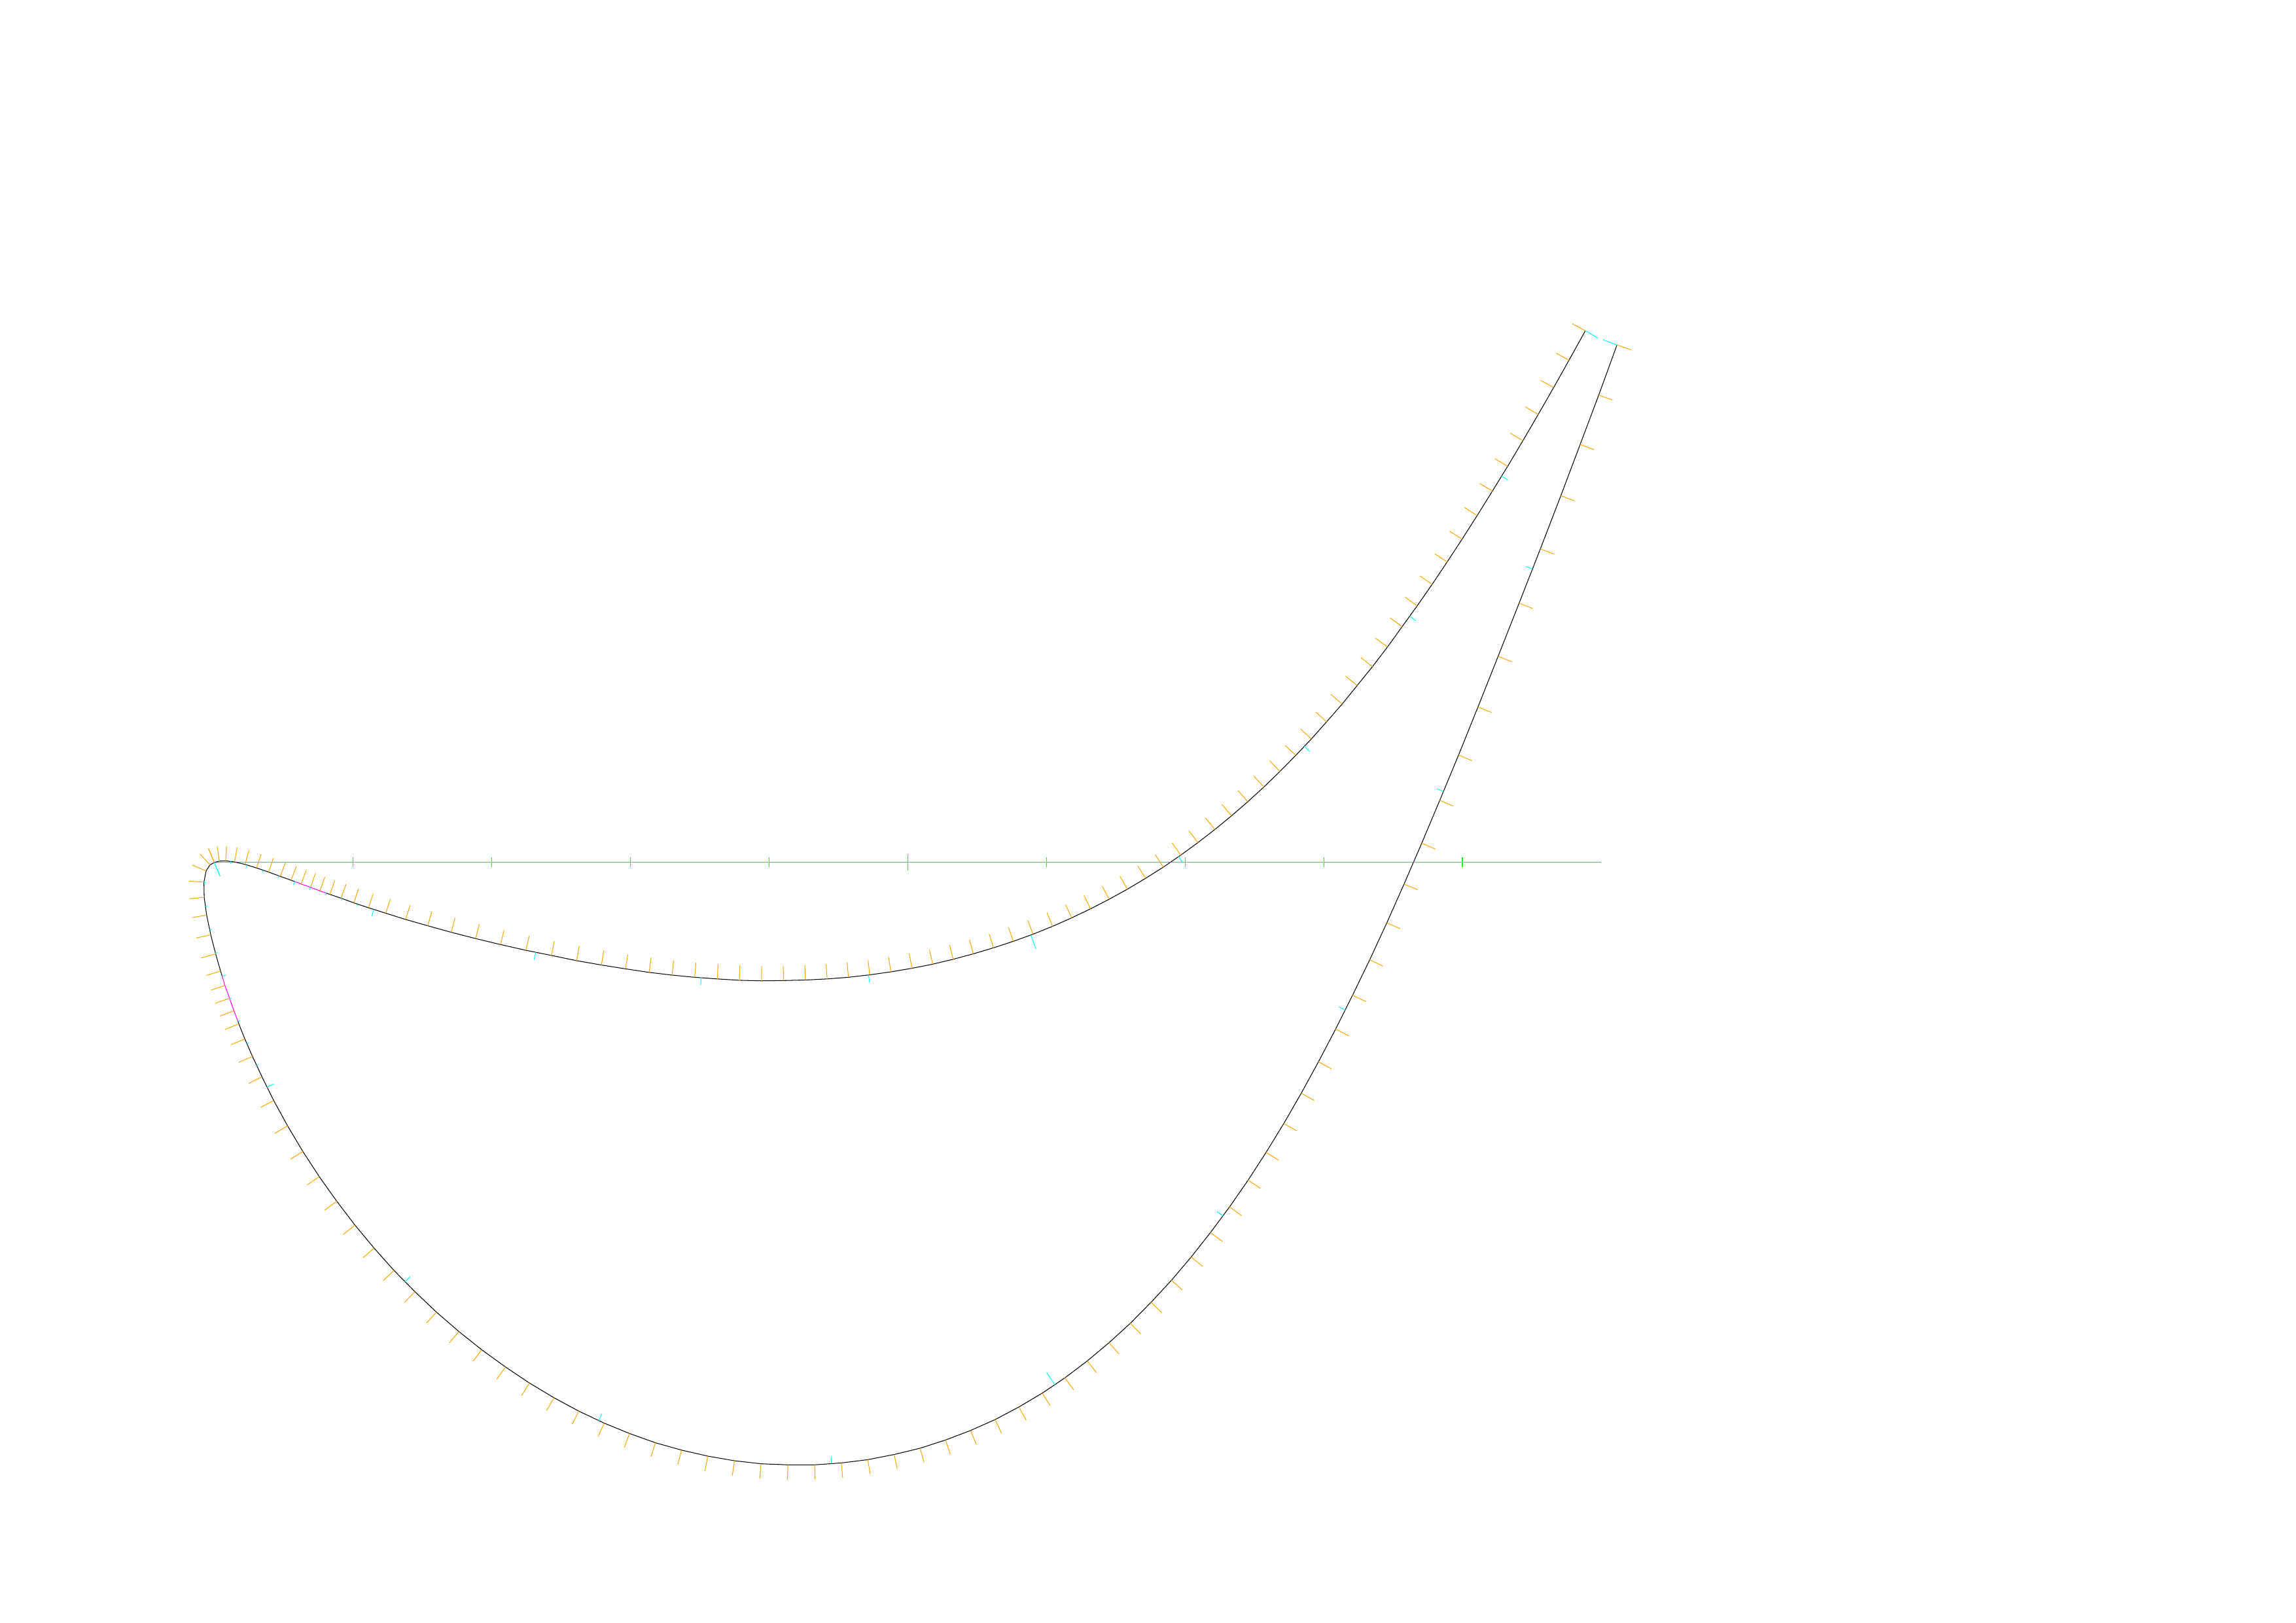
\includegraphics[scale=0.5, trim=0cm 1.5cm 0cm 4cm, clip]{figures/datablade120-2.png}
%     \caption{Spline interpolated blade.}
%     \label{fig:misesBlade}
% \end{figure}

% Once the blade has been approximated with splines, there is an intermediate step for the allocation 
% of the grid properties and the position where the boundary conditions are applied.

% Figure~\ref{fig:misesBCs} represents this intermediate step.

% \begin{figure}[!h]
%     \centering
%     \hspace*{0.6cm}
%     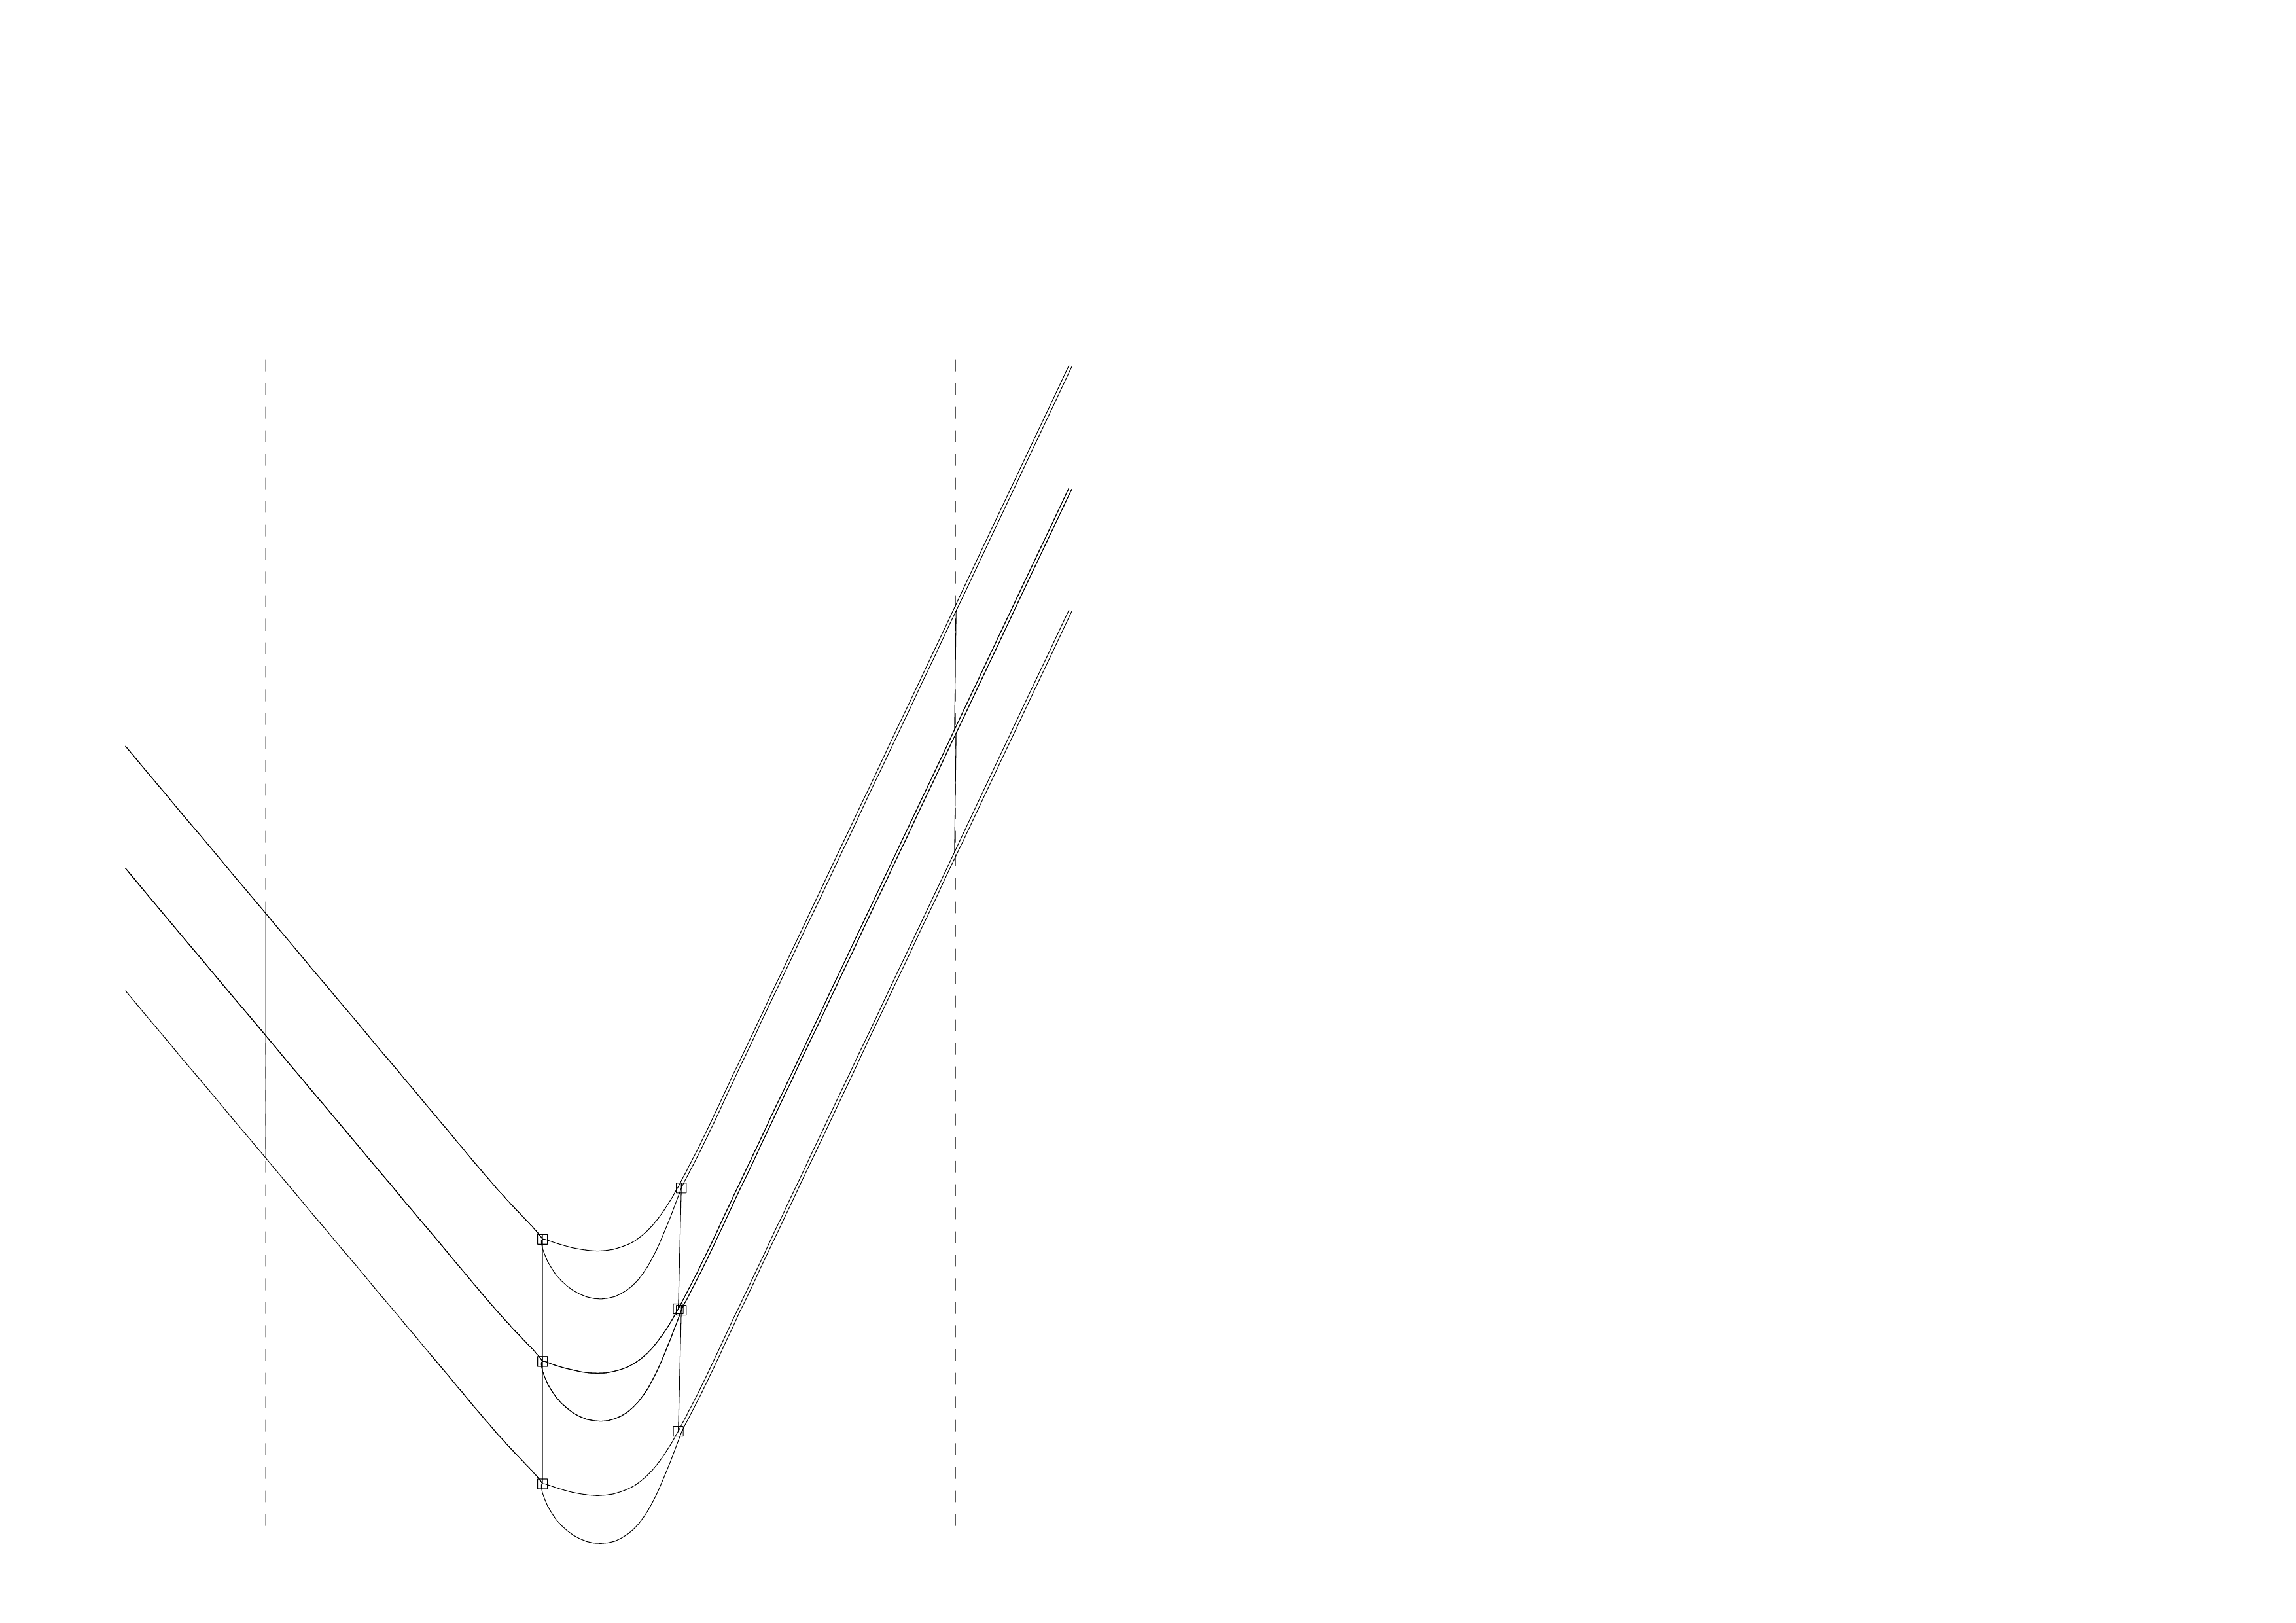
\includegraphics[scale=1, trim=0cm 0cm 0cm 2cm, clip]{figures/datablade120-1.png}
%     \caption{Grid properties allocation and boundary conditions setup.}
%     \label{fig:misesBCs}
% \end{figure}

% The grid as consequently computed using a potential solver which generates an approximation of the flow
% that allows the generation of the study cells inside the domain.

% Figure~\ref{fig:misesGrid} shows the grid used in the present work. 
% The grid features a \textbf{H-type} grid both at the inlet and the outlet of the blade.
% The reason of using this grid type relies in the accuracy of results and the appreciable 
% speed up with respect to the \textbf{I-type} grids. 

% \begin{figure}[!h]
%     \centering
%     \hspace*{-1cm}
%     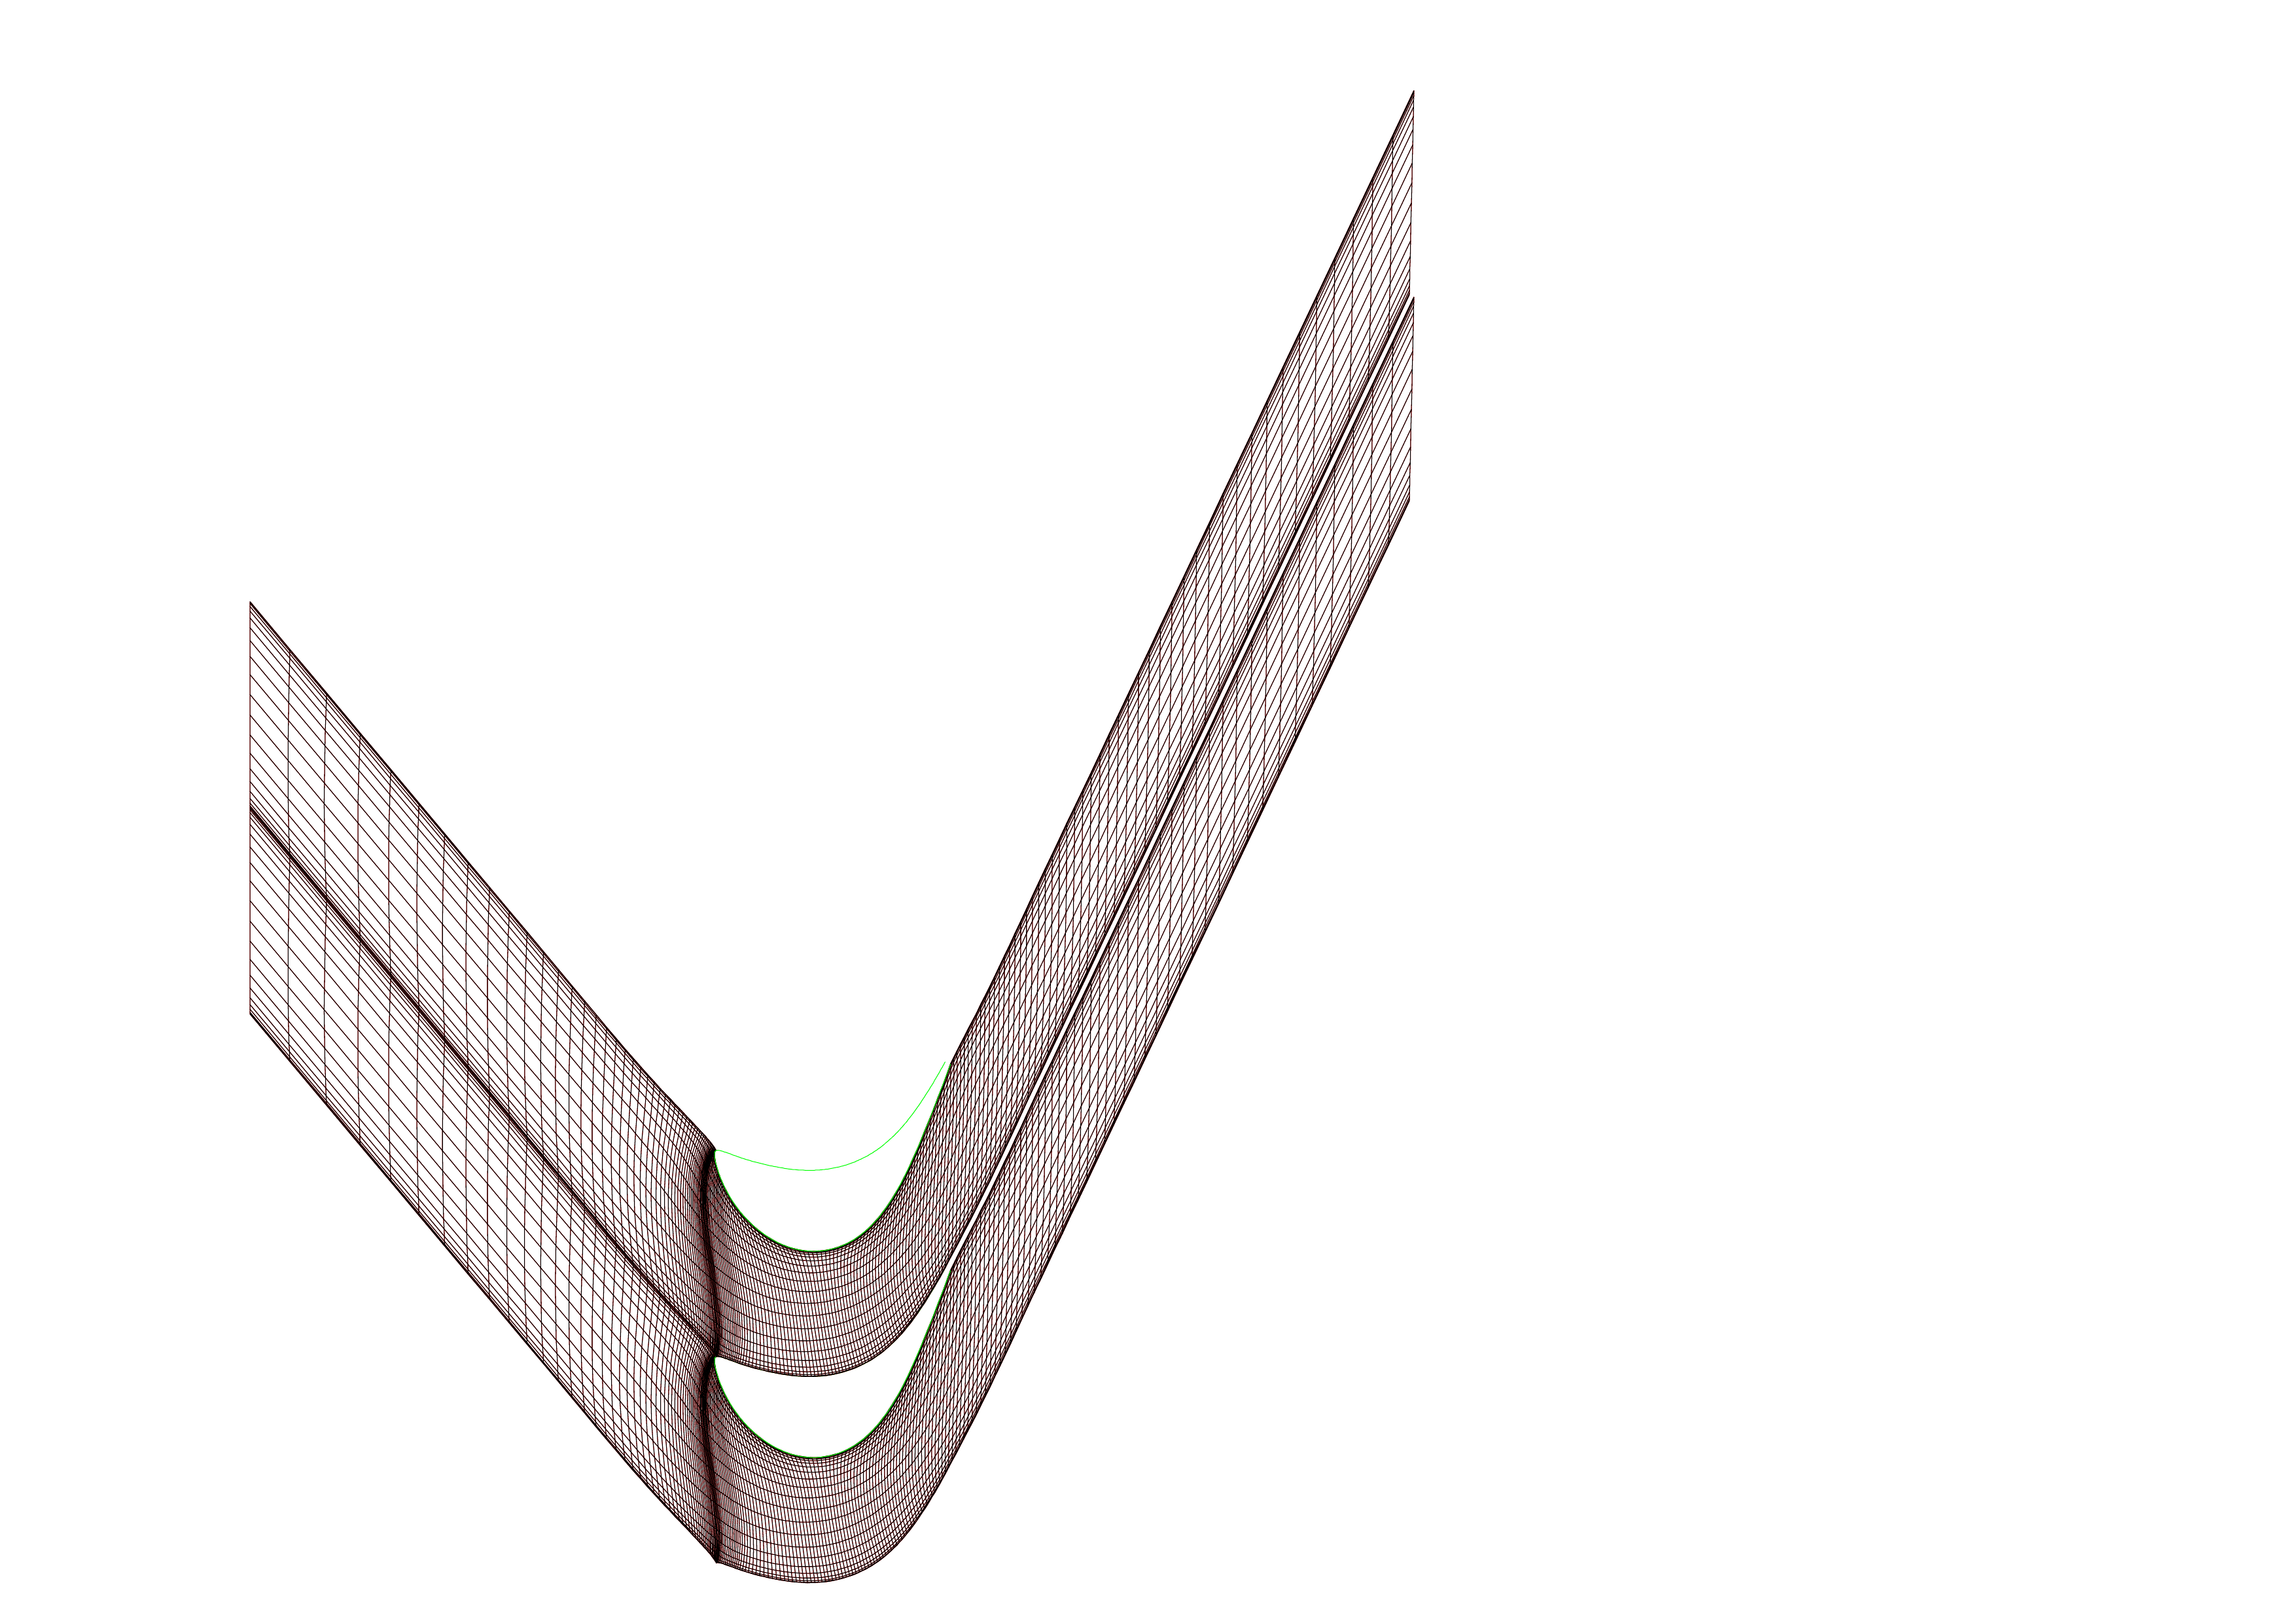
\includegraphics[scale=0.87]{figures/datablade120-3.png}
%     \caption{Grid used by \texttt{ISES} for the computation of the flow properties.}
%     \label{fig:misesGrid}
% \end{figure}

% The flow properties are computed in \texttt{ISES} following \texttt{ises.datablade} properties.

% Figure~\ref{fig:misesFlow} shows the flow properties inside the blade channels.

% \begin{figure}[!h]
%     \centering
%     \hspace*{-2cm}
%     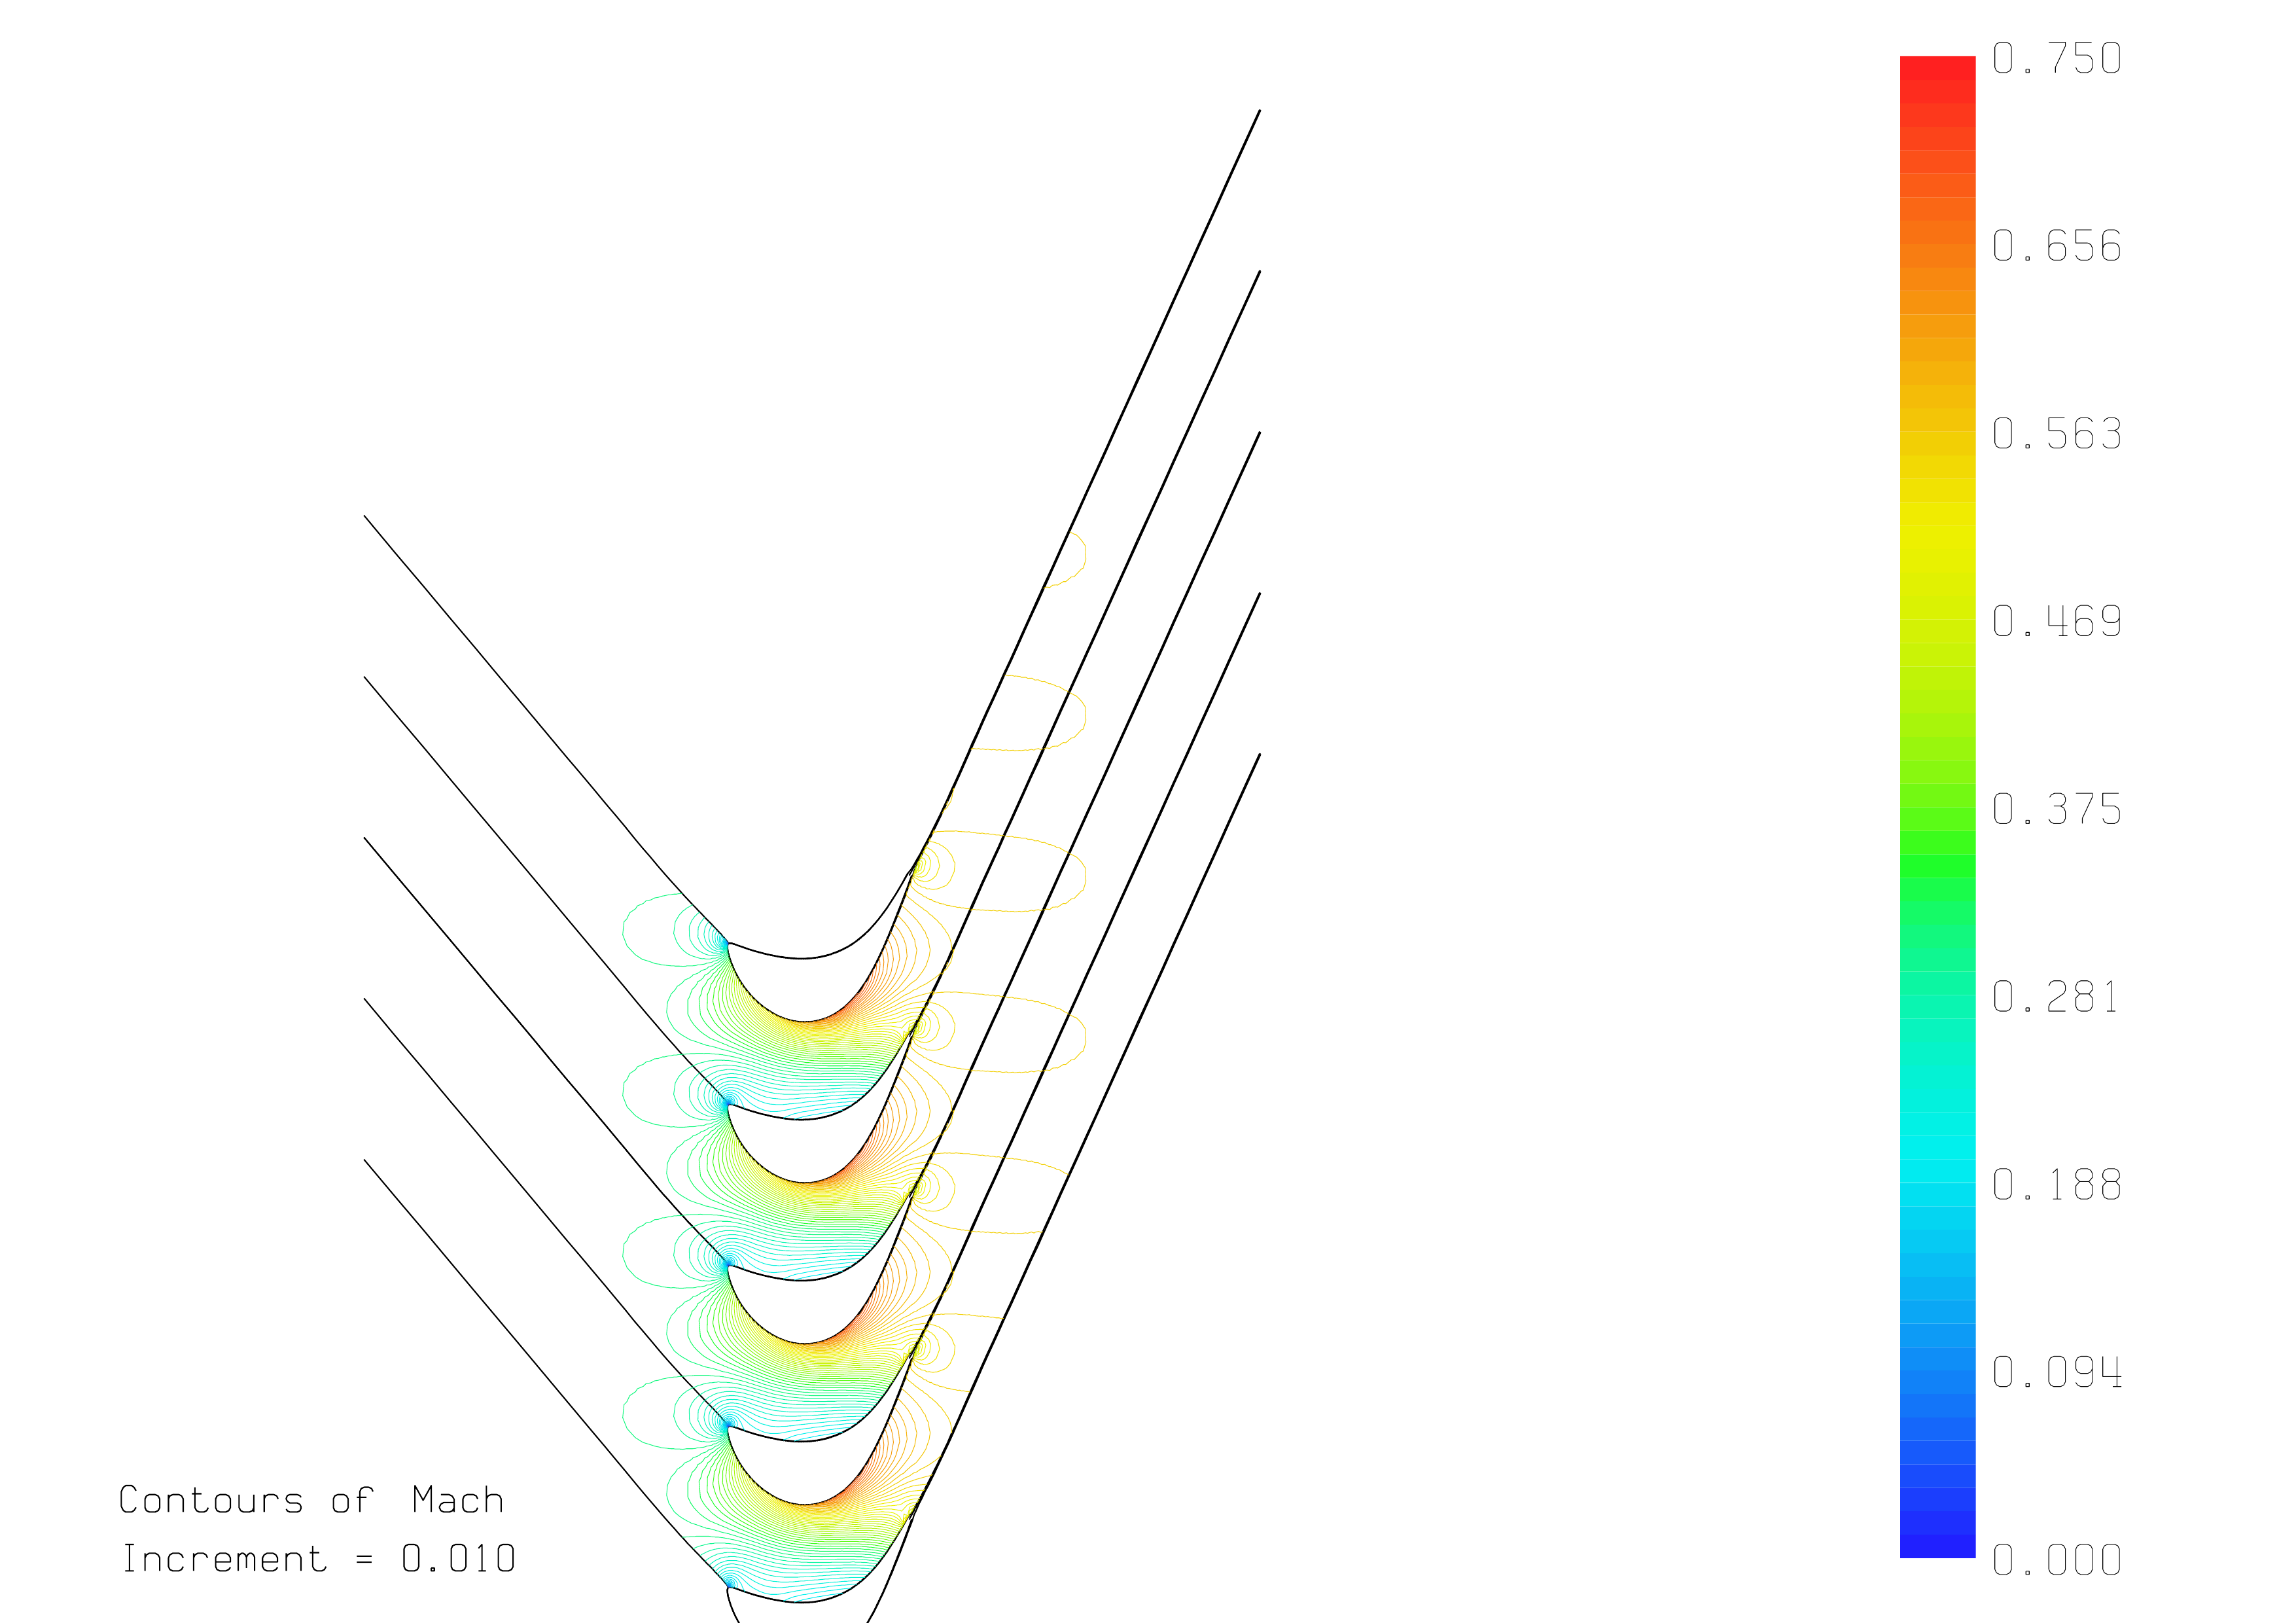
\includegraphics[scale=0.75]{figures/datablade120-4.png}
%     \caption{Countour plot of the flow properties computed by \texttt{ISES} module.}
%     \label{fig:misesFlow}
% \end{figure}

% Once computed the flow, the Mach fraction distribution along the blade is extracted using 
% the \texttt{EDP} module in \texttt{MISES}. This module reads the selected flow property - in this case 
% the Mach number - and saves it inside a \texttt{.dat} file. From this file, it is possible 
% to compute the Mach fraction distribution along the blade by just taking the two Mach number 
% at the trailing edge of the blade (they are slightly different because the presence of the wake) and 
% computing both the Mach fraction distribution at the suction side and at the pressure side of the blade.

Figure~\ref{fig:misesBlade} displays a blade pre-processed by \texttt{ISET} for a spline interpolation of the geometry. This can be seen as the preprocessing for the grid generation of the
problem

\begin{figure}[!h]
    \centering
    \hspace*{2cm}
    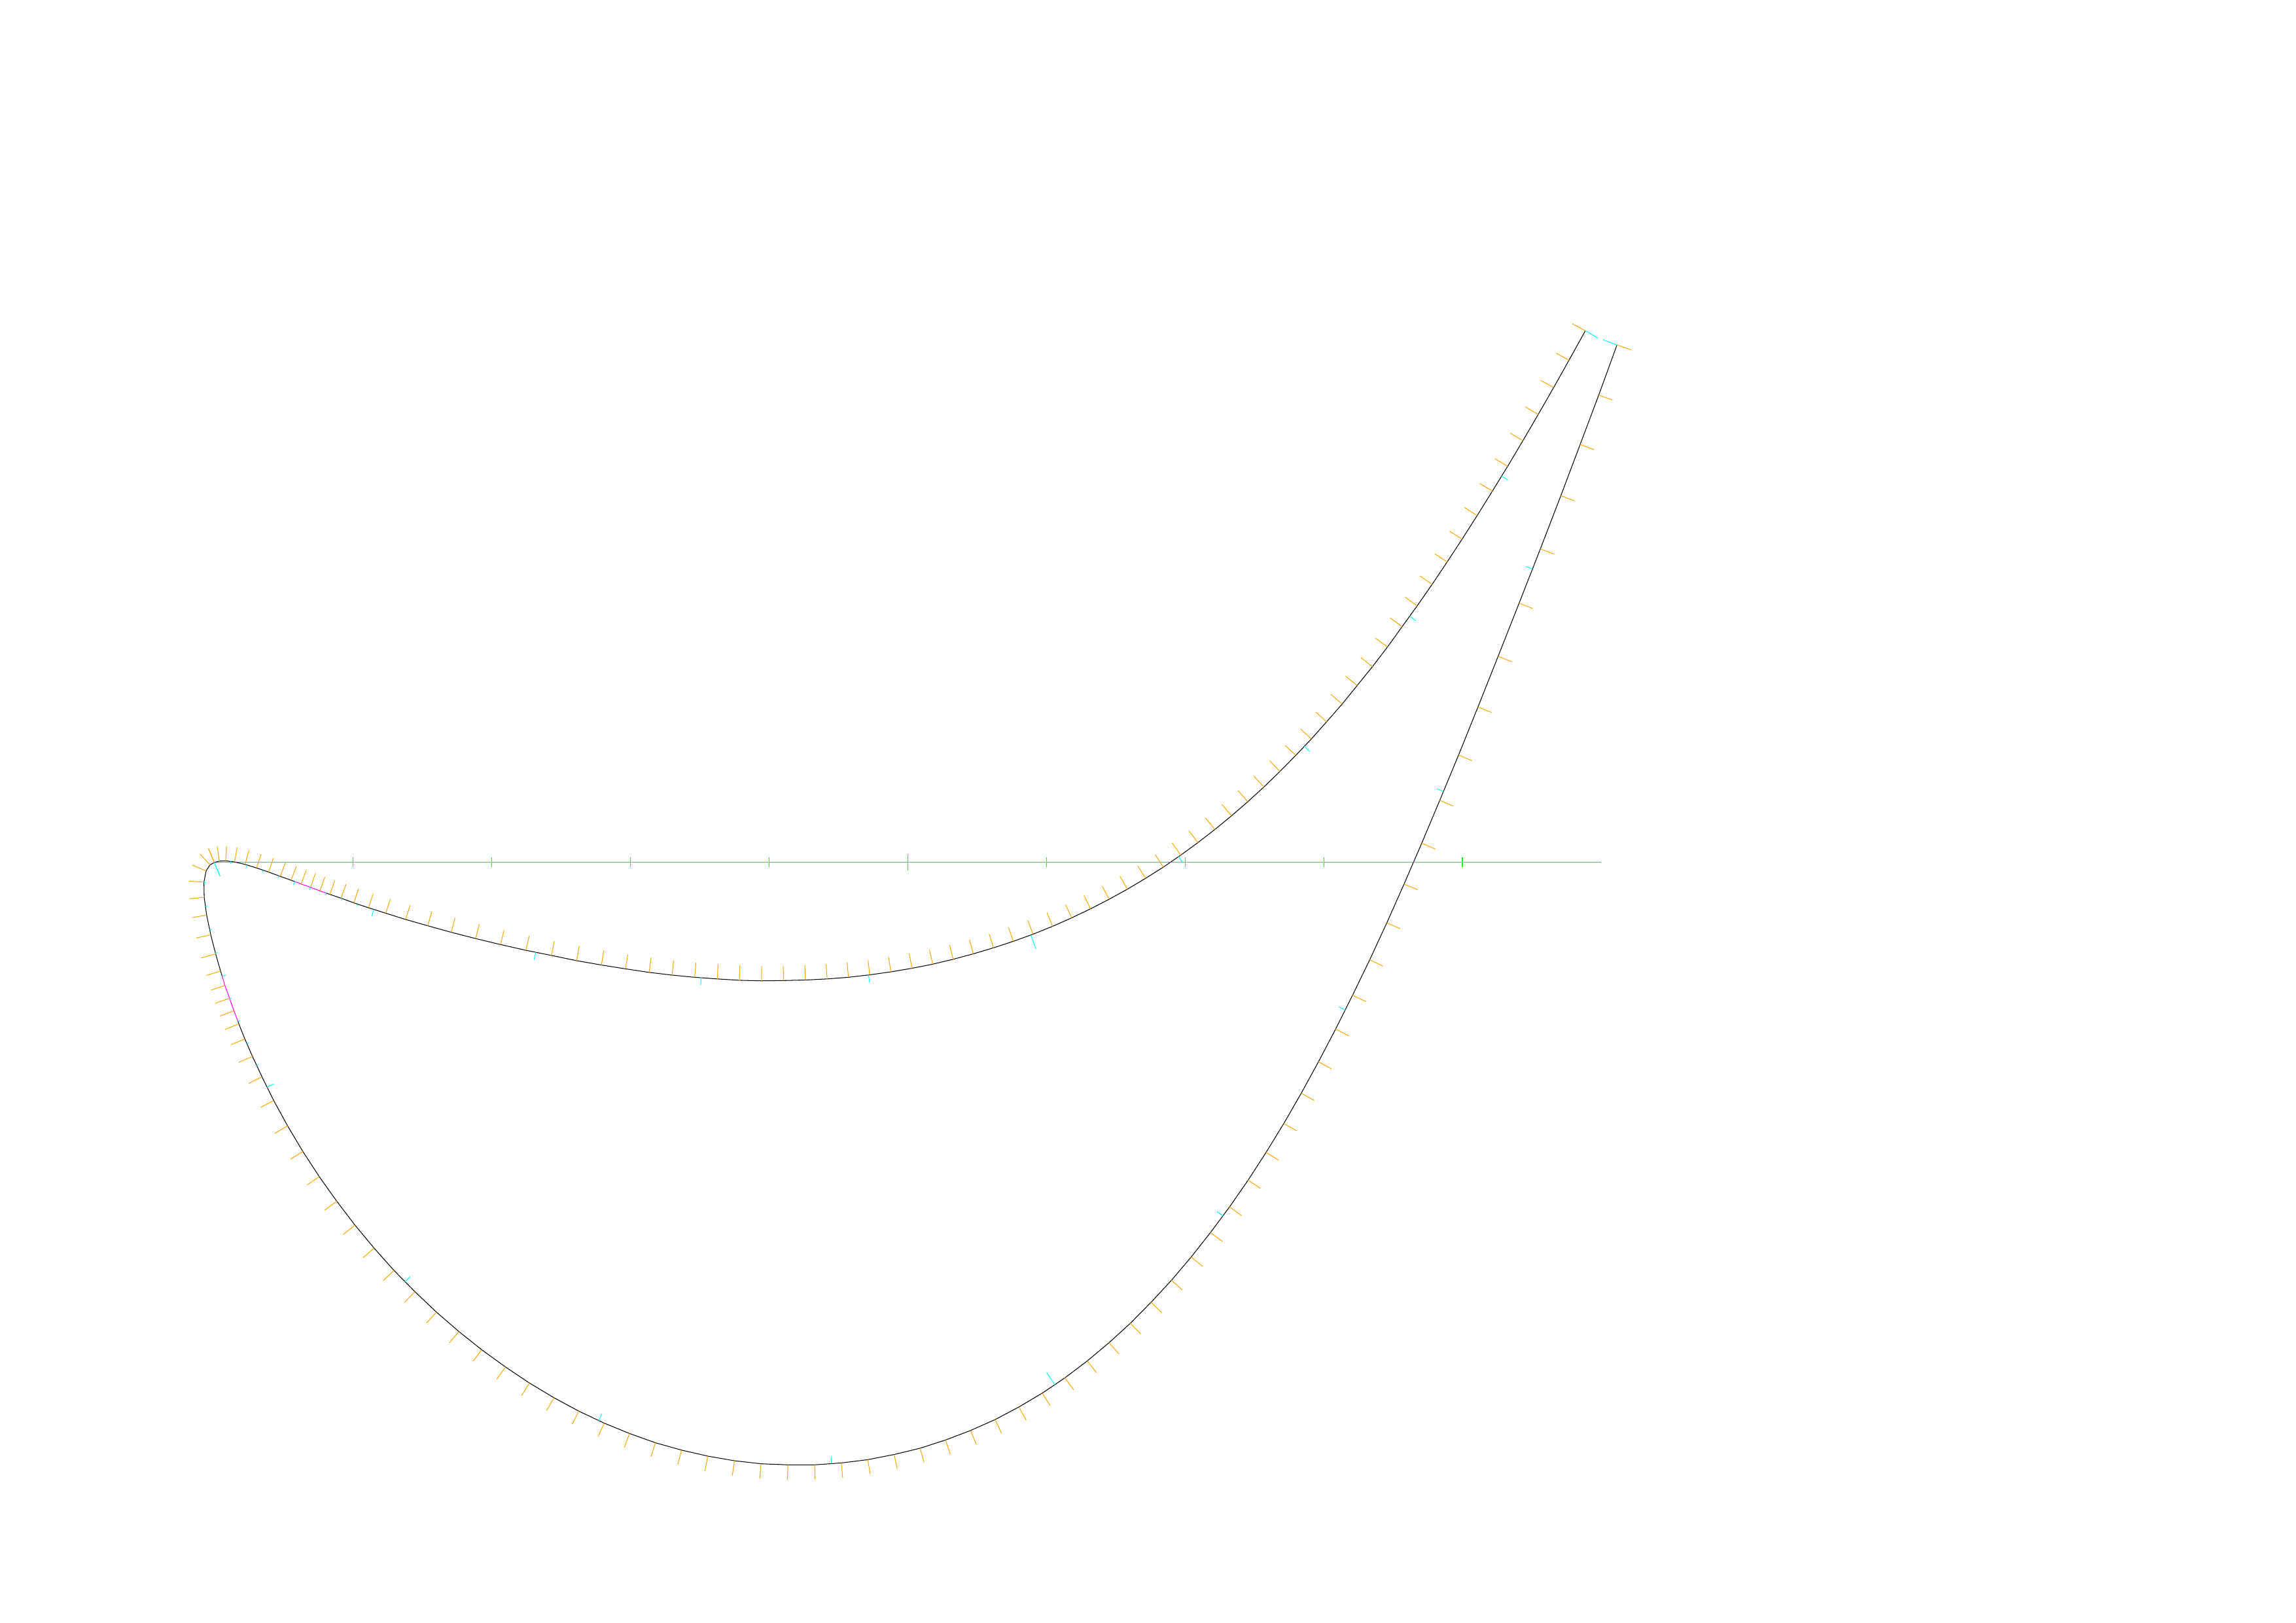
\includegraphics[scale=0.4, trim=0cm 1.5cm 0cm 4cm, clip]{figures/datablade120-2.png}
    \caption{Spline-interpolated blade.}
    \label{fig:misesBlade}
\end{figure}

Following the spline approximation, there is an intermediate step for allocating the grid properties and defining the position of the boundary conditions, as shown in Figure~\ref{fig:misesBCs}.

\begin{figure}[H]
    \centering
    \hspace*{0.6cm}
    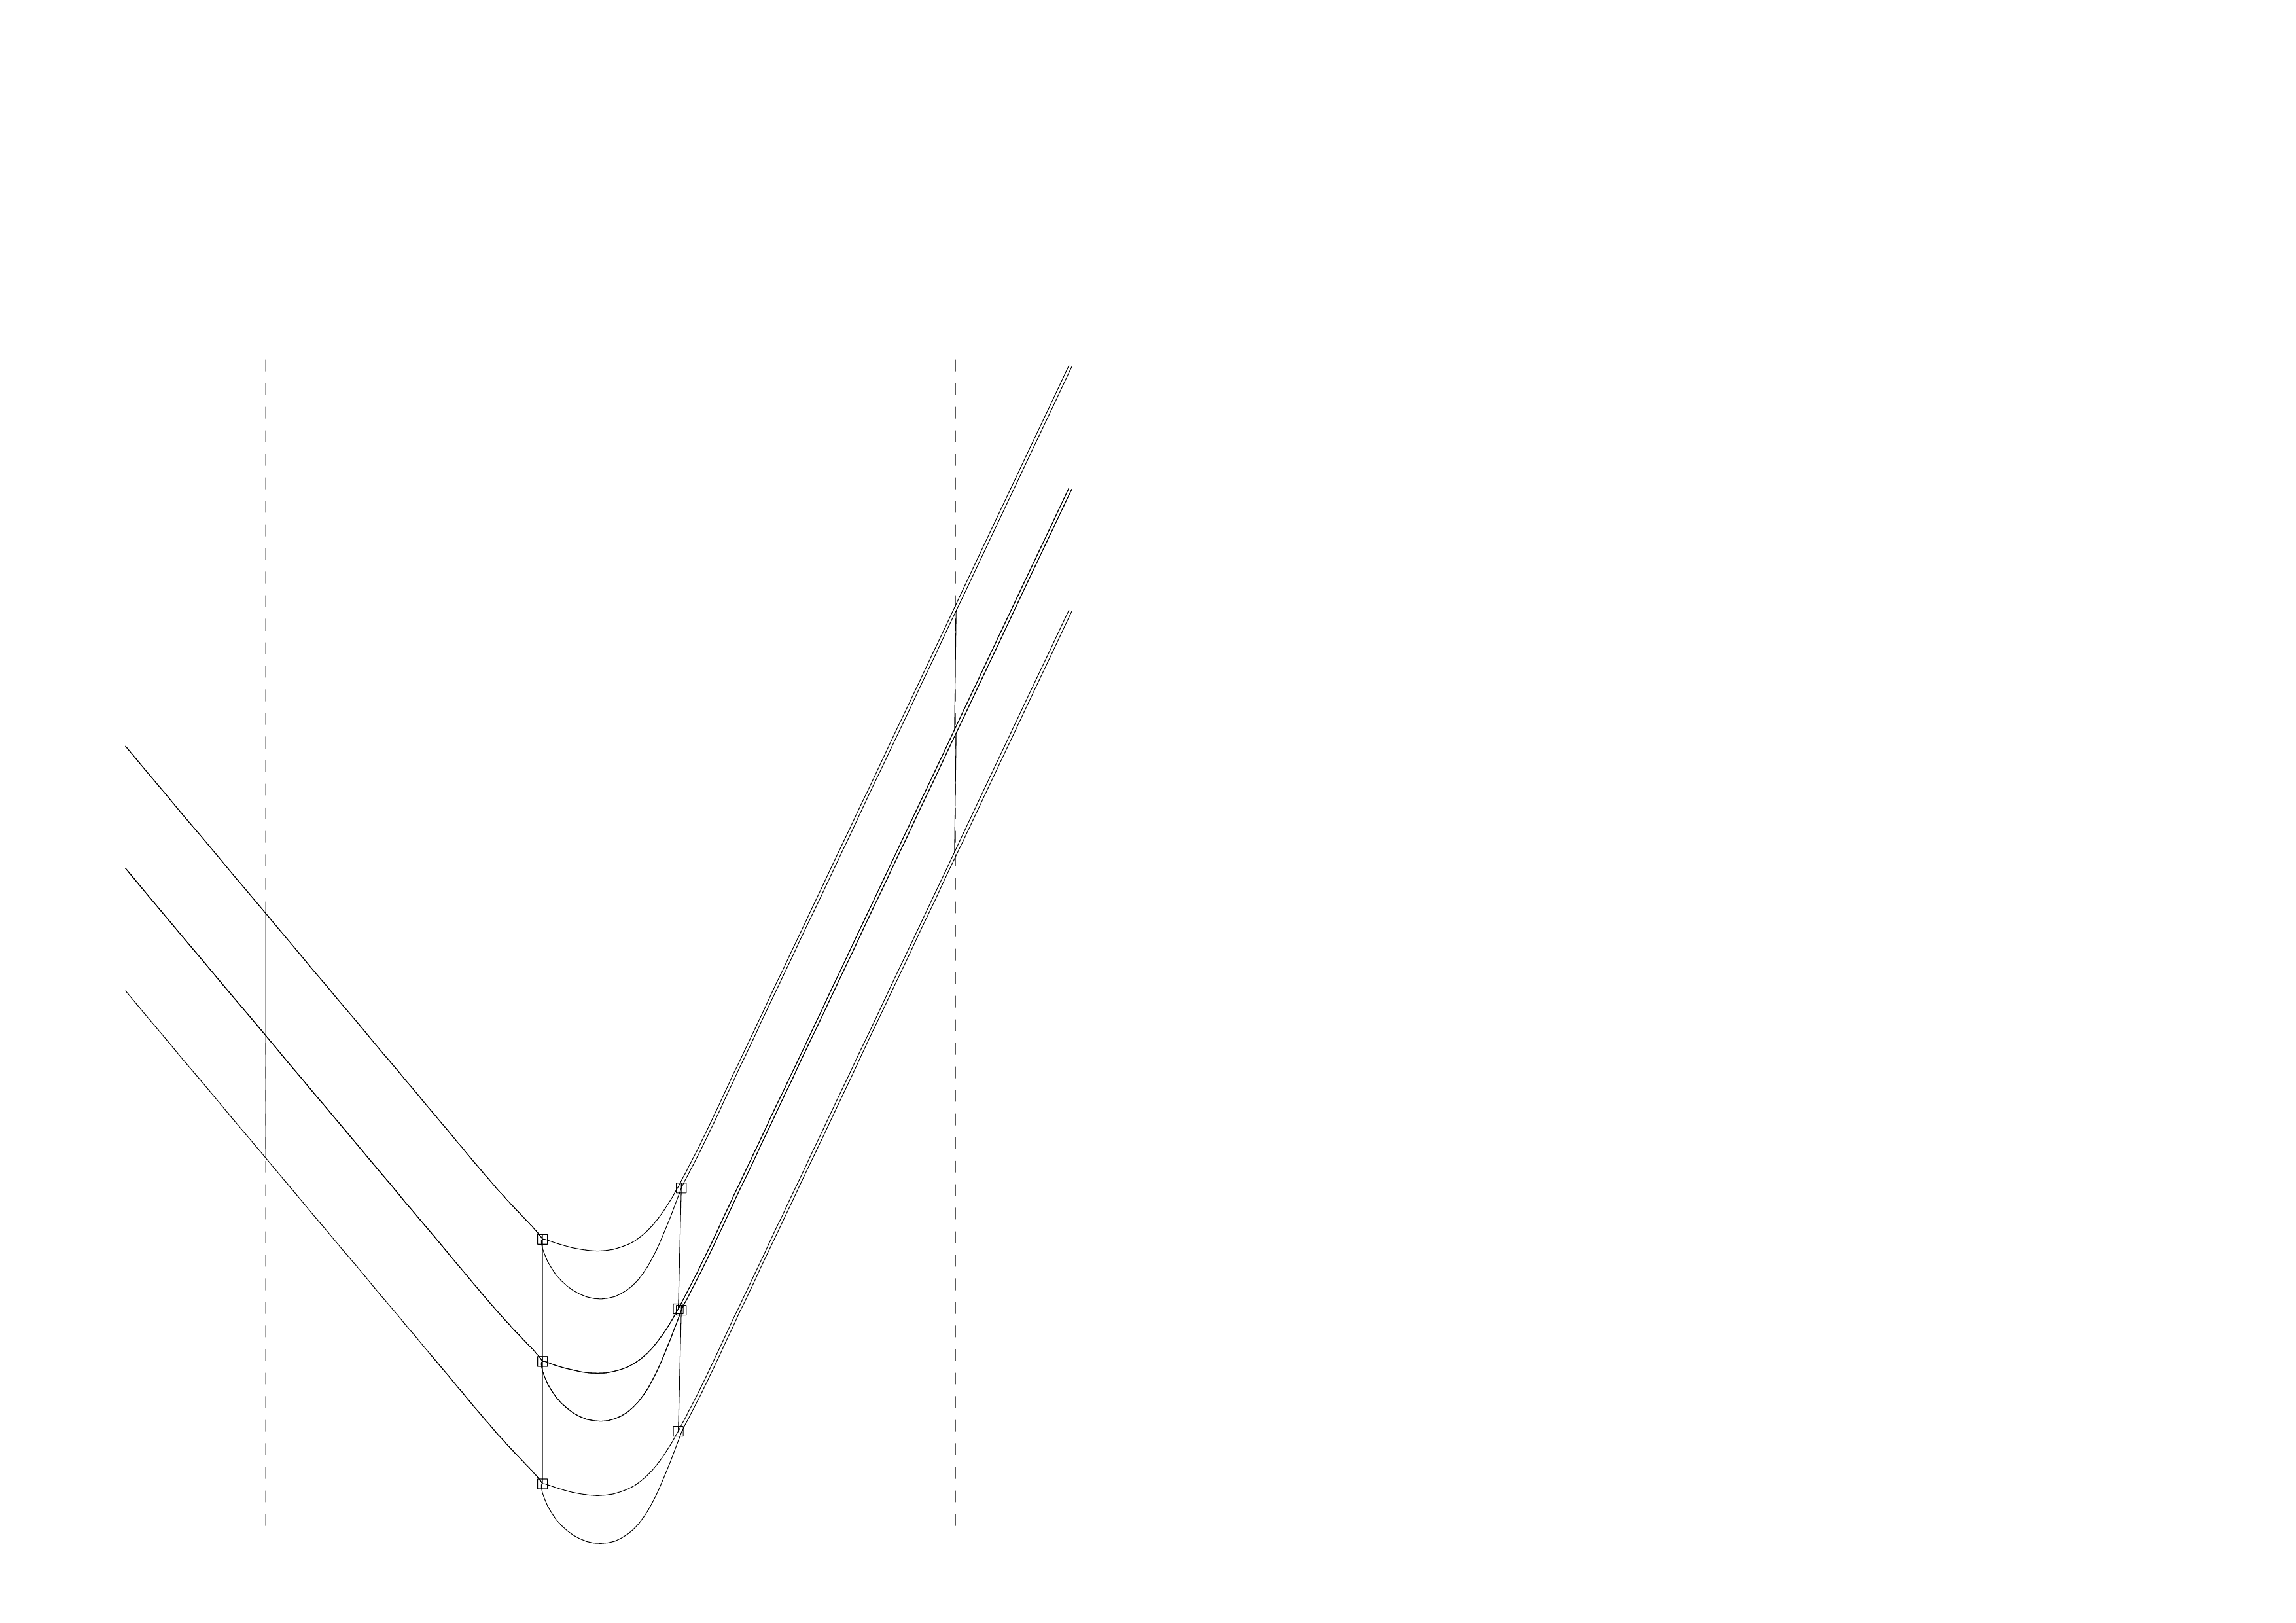
\includegraphics[scale=1, trim=0cm 0cm 0cm 2cm, clip]{figures/datablade120-1.png}
    \caption{Grid properties allocation and boundary conditions setup.}
    \label{fig:misesBCs}
\end{figure}

The grid is consequently computed using a potential solver which generates an approxi-
mation of the flow that allows the generation of the study cells inside the domain.

\begin{figure}[H]
    \centering
    \hspace*{-1cm}
    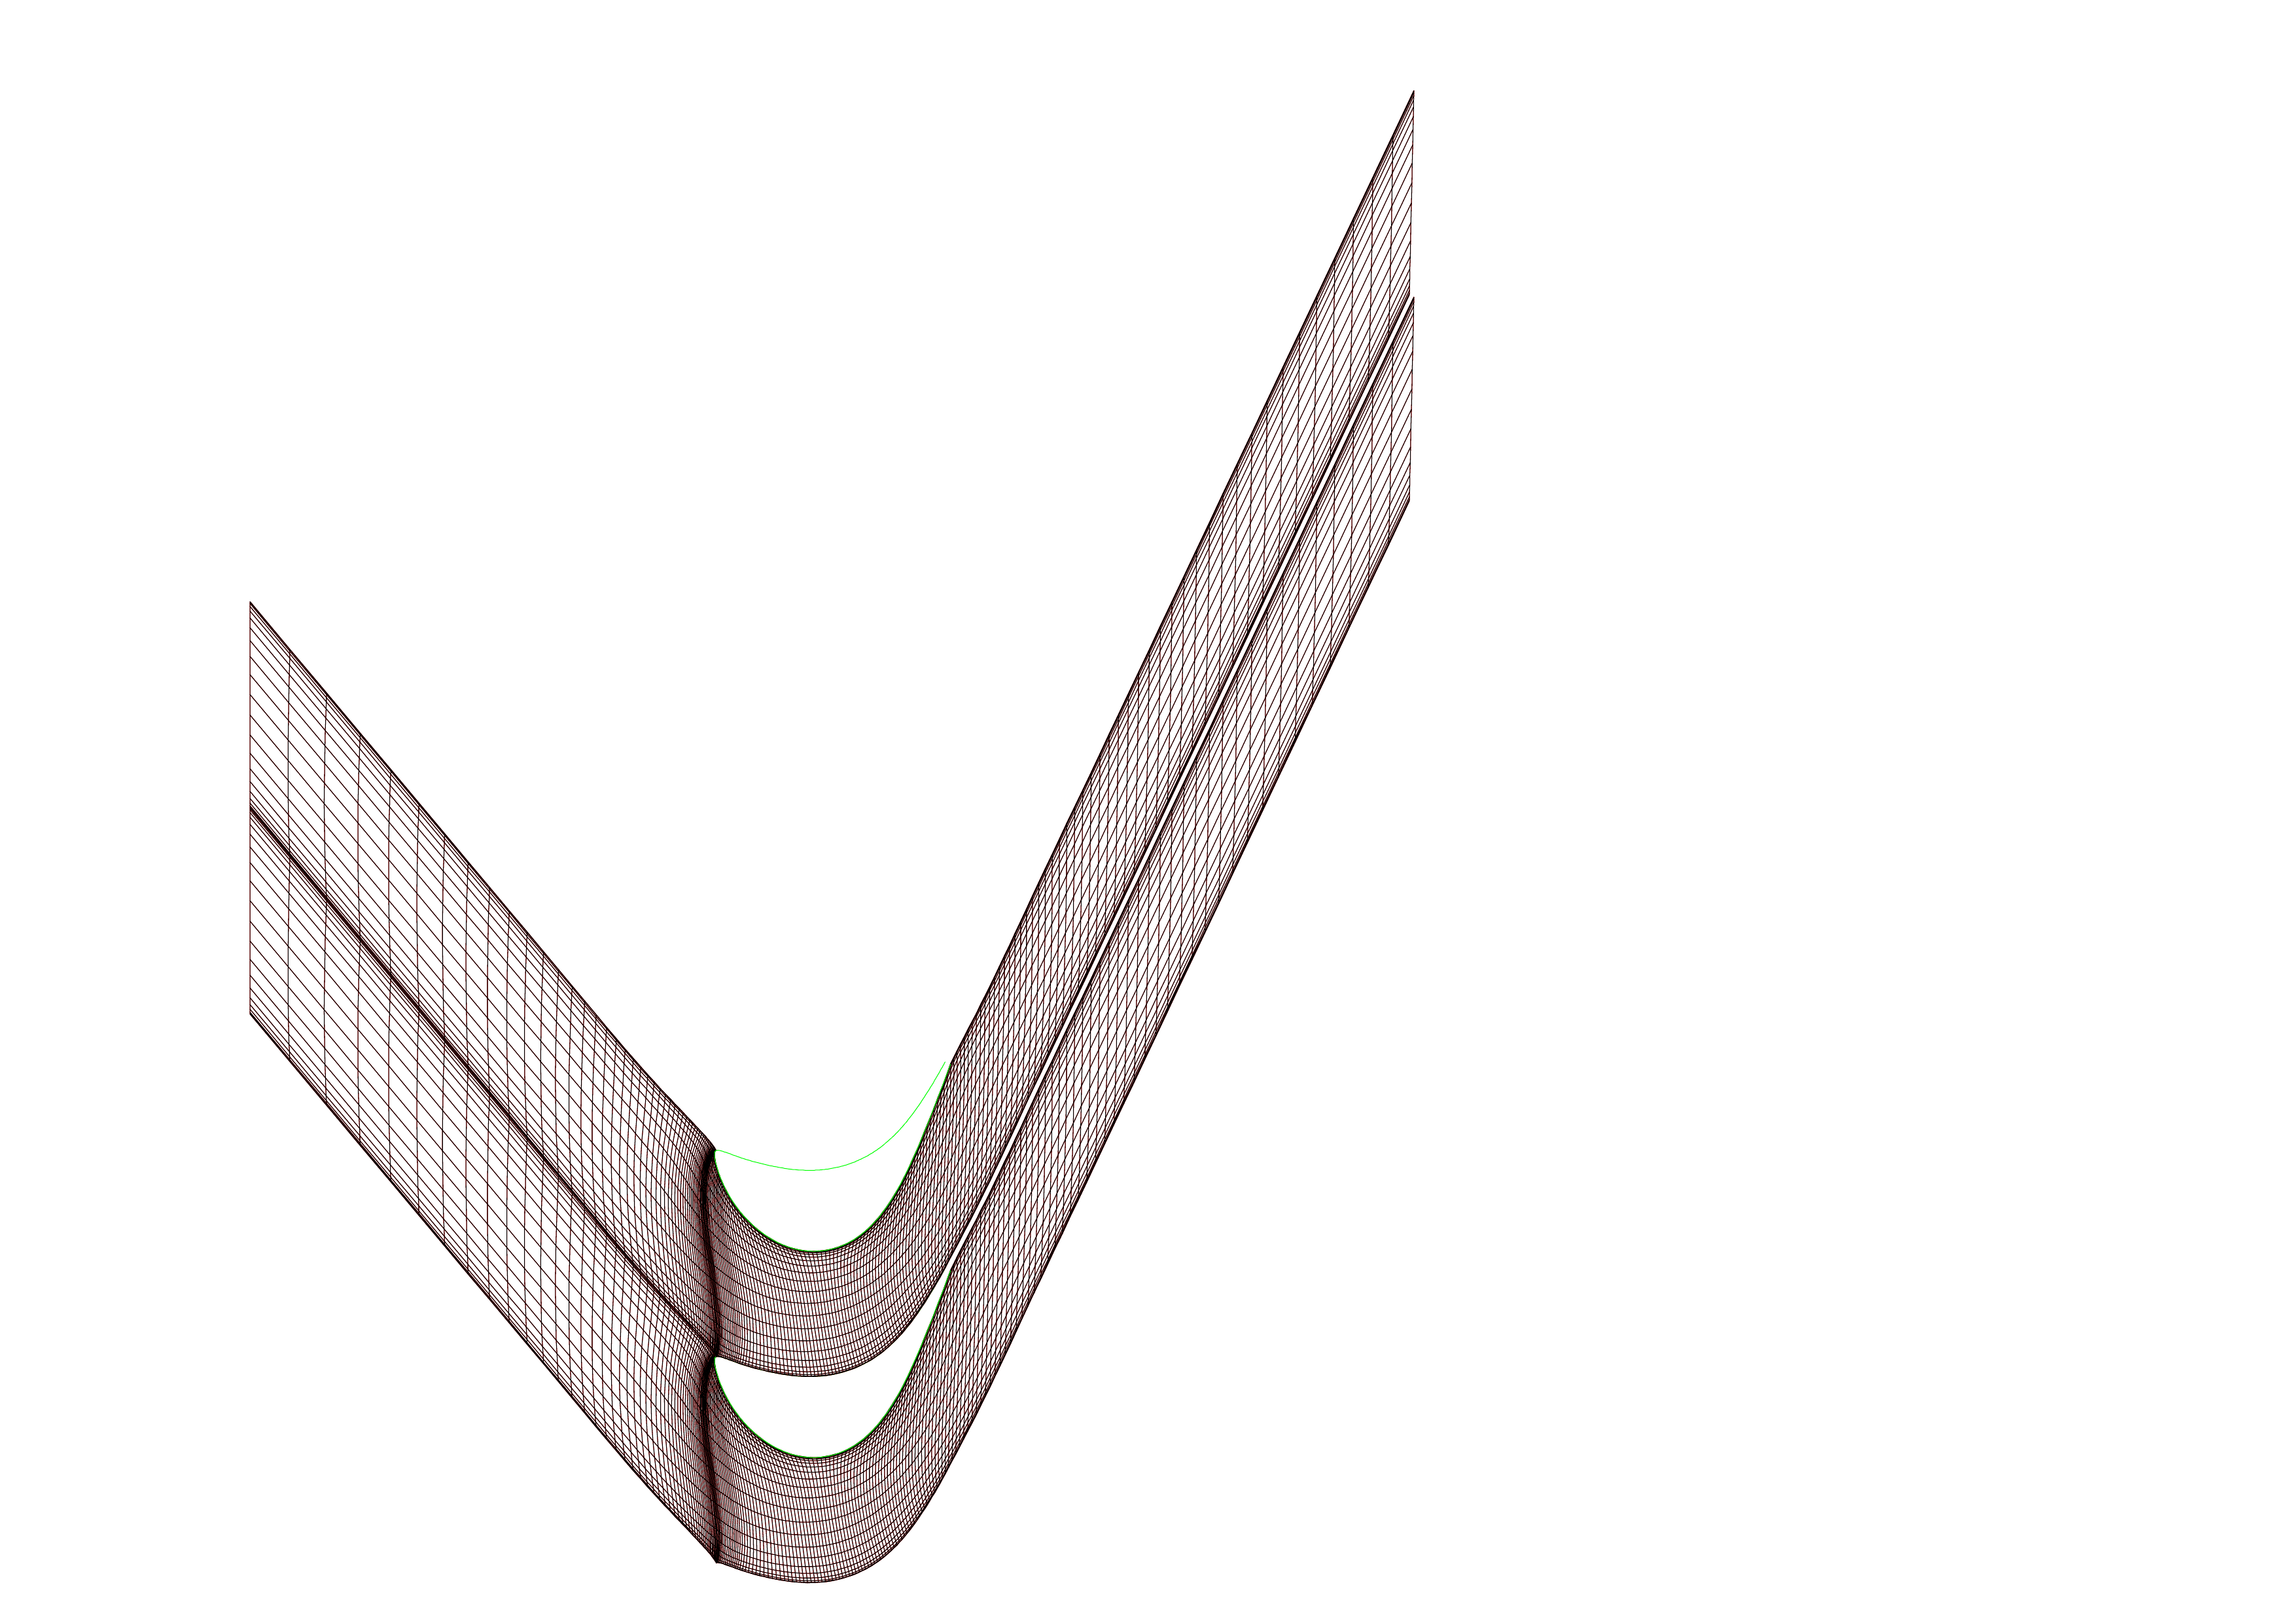
\includegraphics[scale=0.87]{figures/datablade120-3.png}
    \caption{Grid used by \texttt{ISES} for flow property computation.}
    \label{fig:misesGrid}
\end{figure}

Flow properties are computed in \texttt{ISES} based on \texttt{ises.datablade} settings, as visualized in Figure~\ref{fig:misesFlow}.

\begin{figure}[H]
    \centering
    % \hspace*{-2cm}
    % 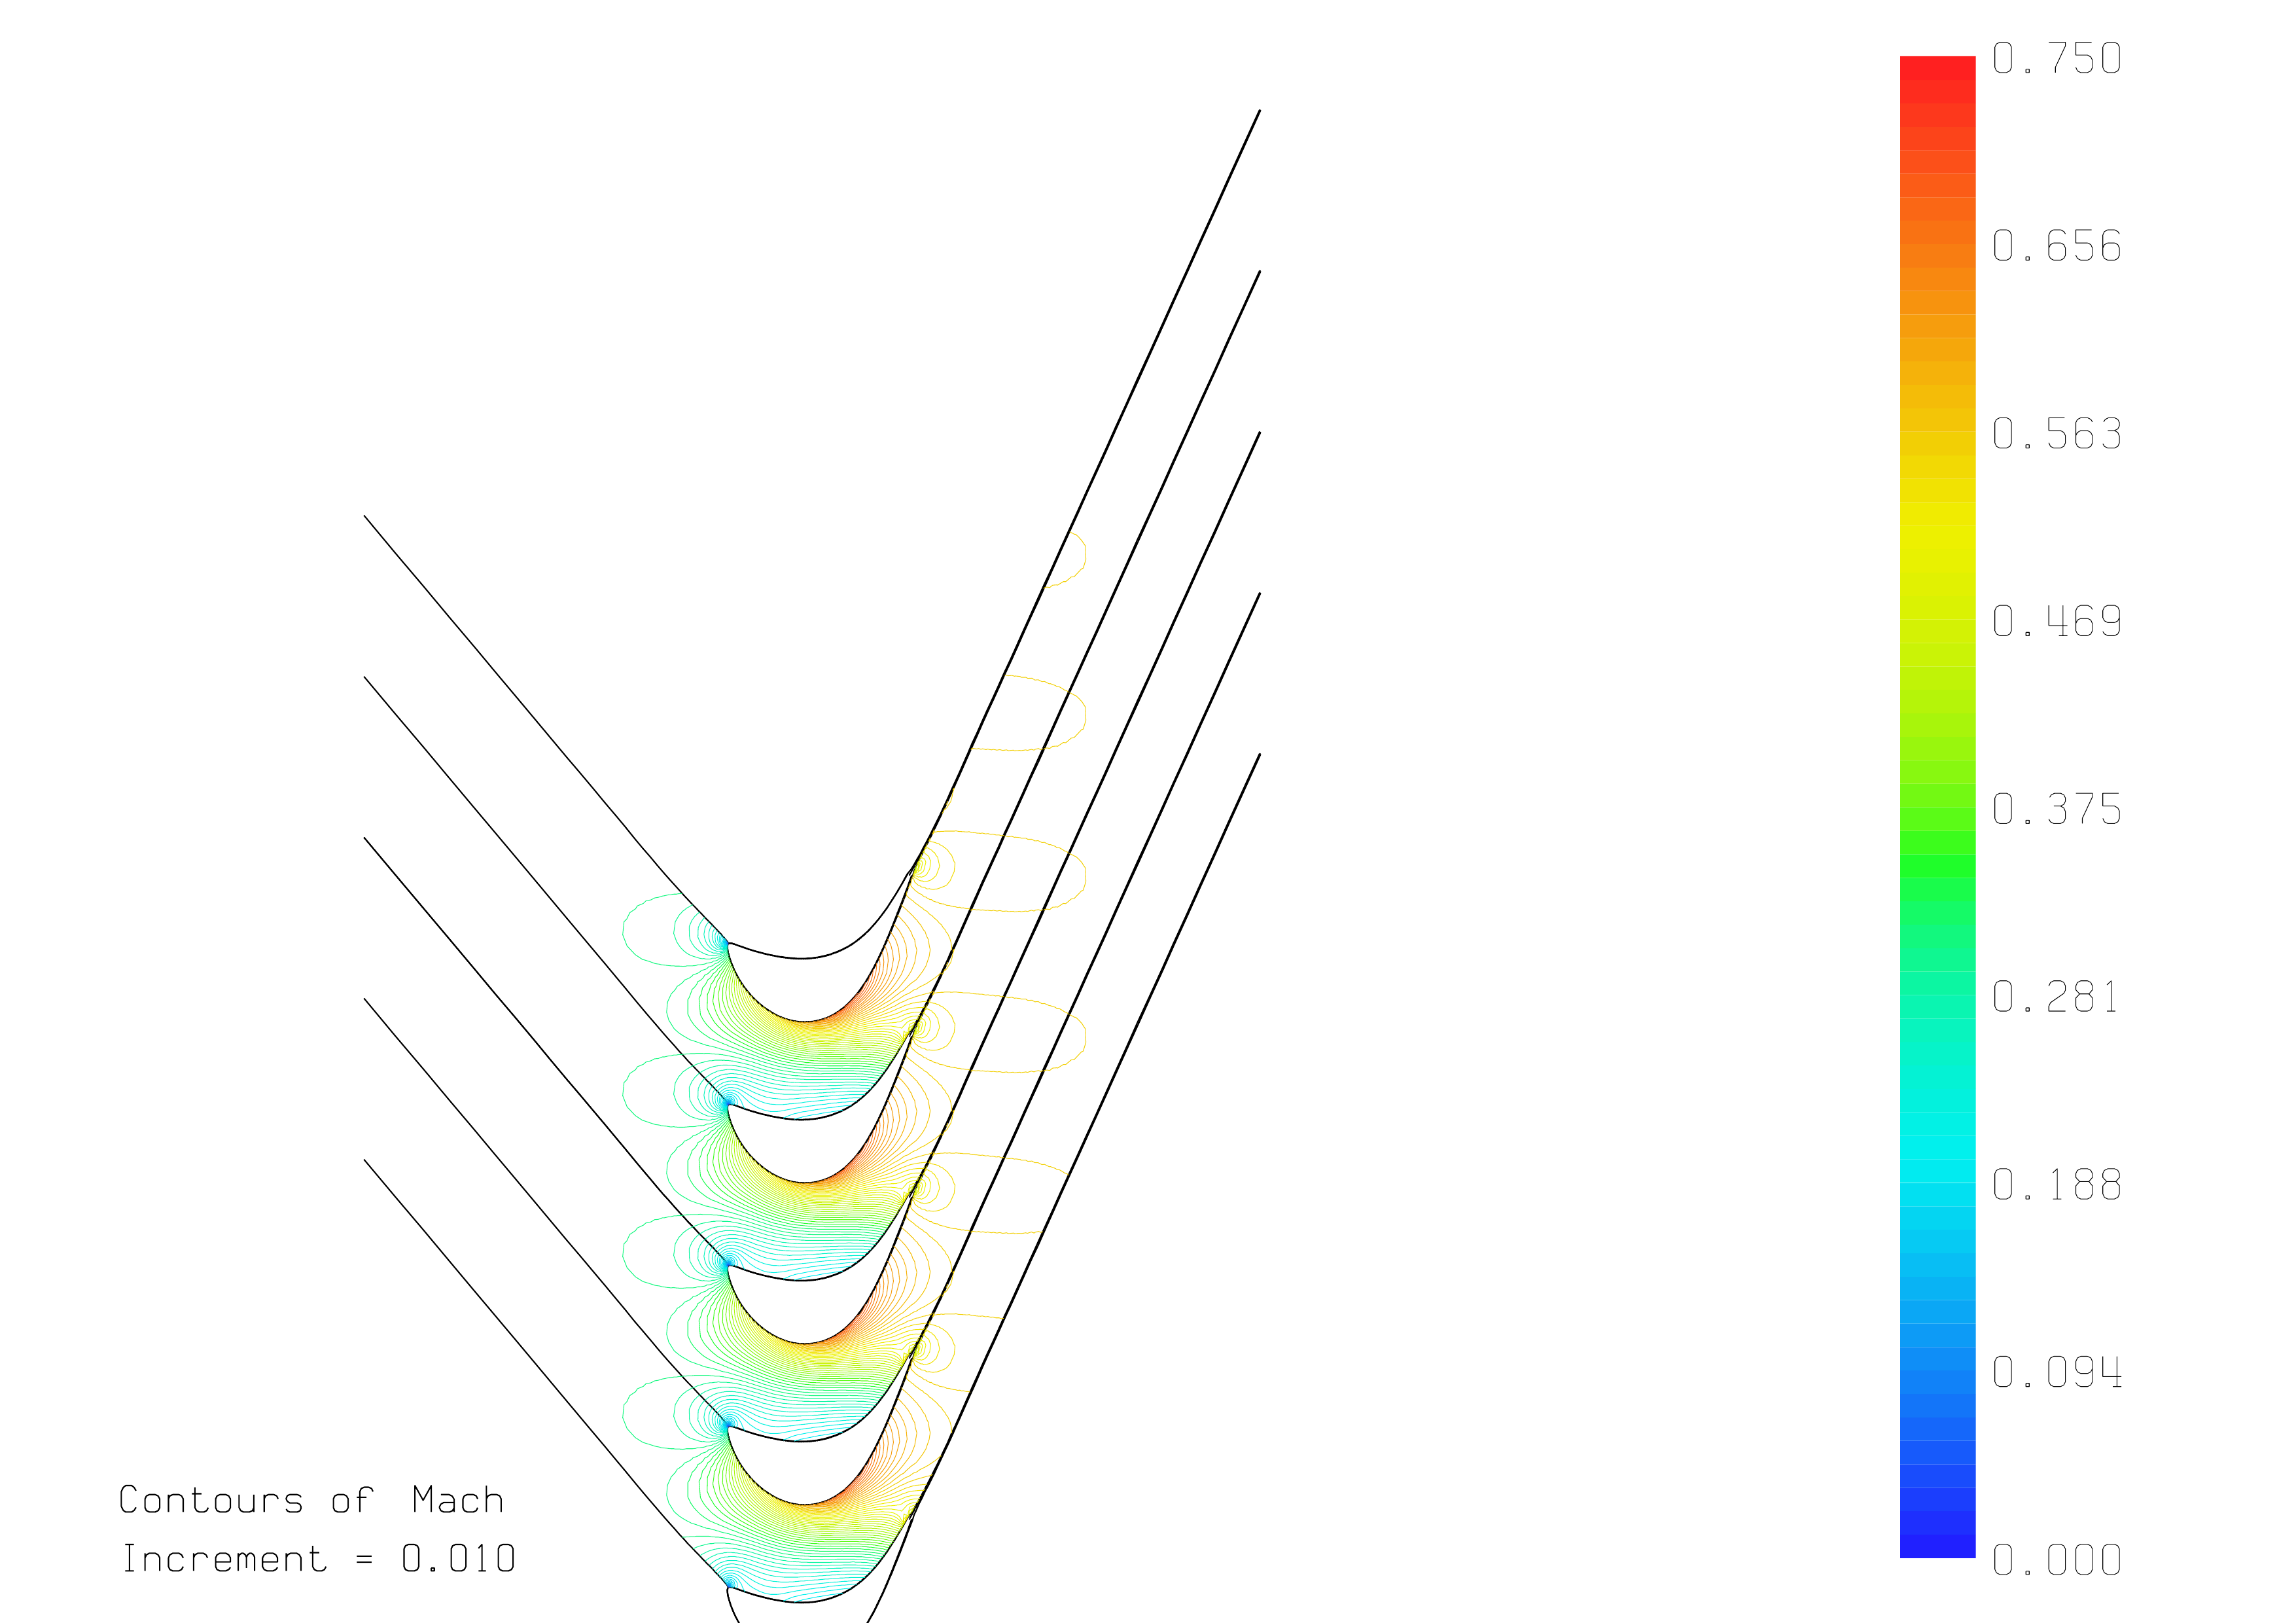
\includegraphics[scale=0.75]{figures/datablade120-4.png}
    \hspace*{-0.5cm}
    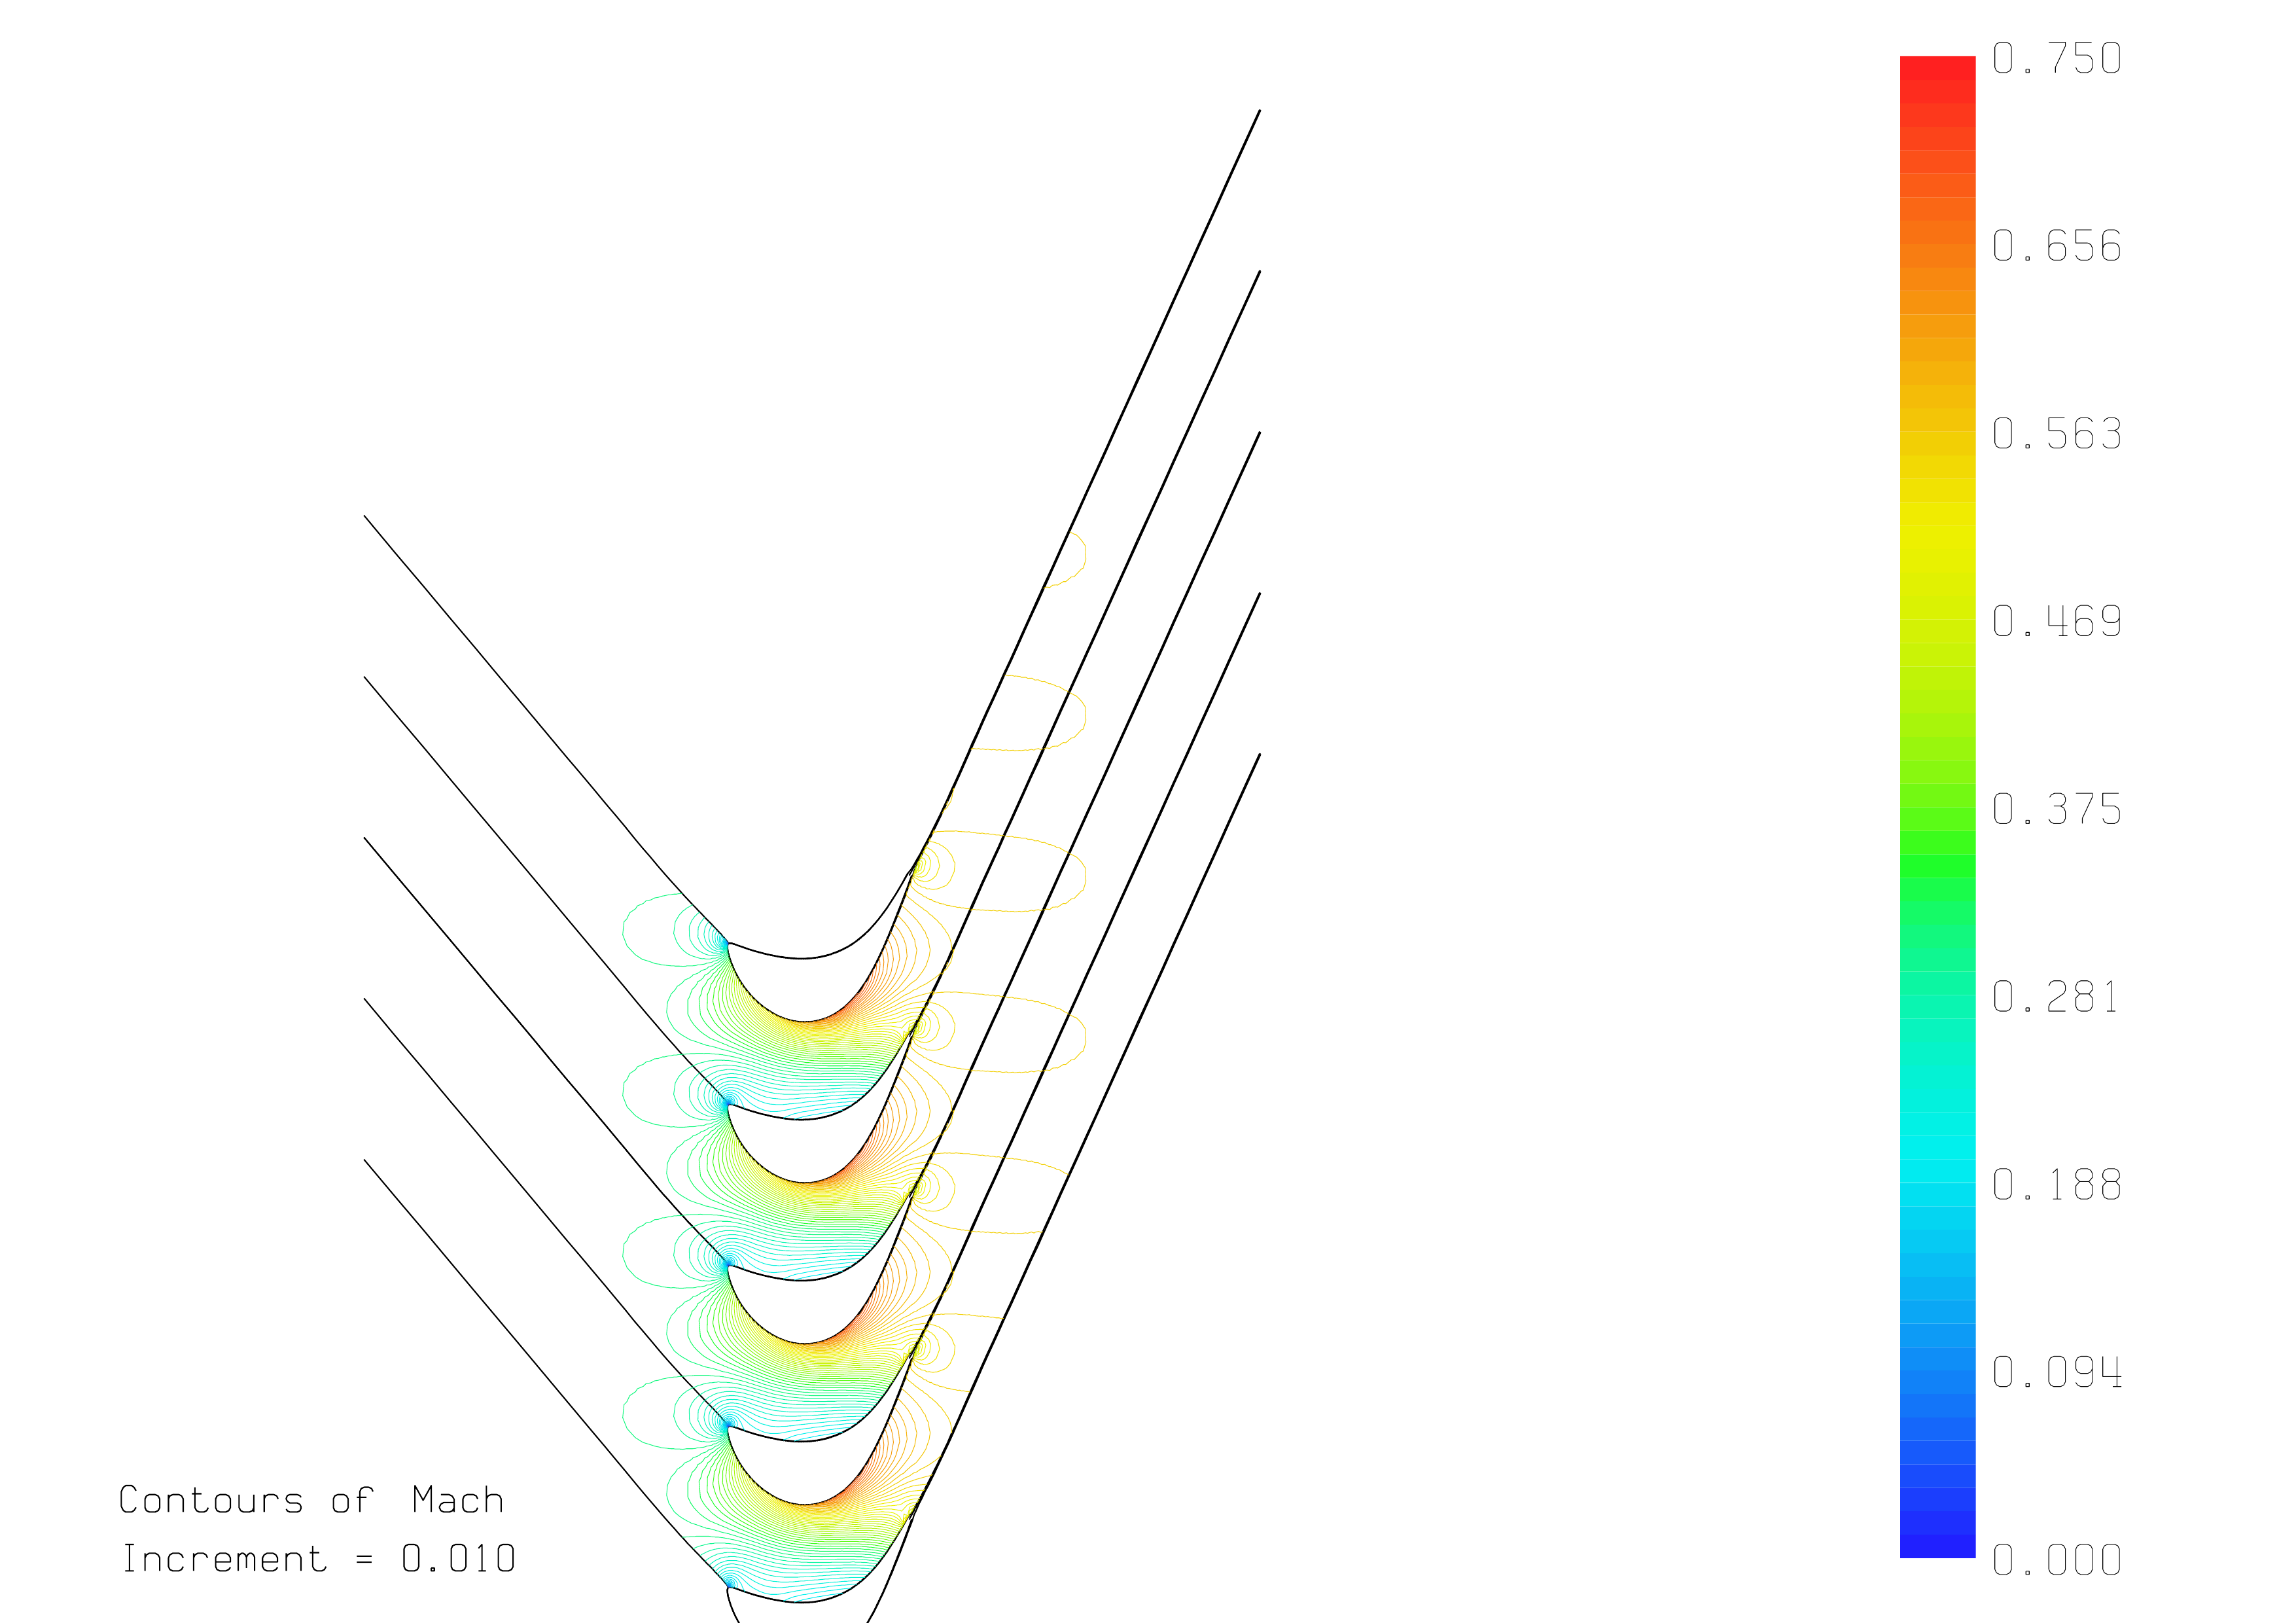
\includegraphics[width=1.1\textwidth]{figures/datablade120-4.png}
    \caption{Contour plot of flow properties computed by \texttt{ISES} module.}
    \label{fig:misesFlow}
\end{figure}

Once flow is computed, the Mach fraction distribution along the blade is extracted using the \texttt{EDP} module in \texttt{MISES}. 
This module reads selected flow property (Mach number in this case) and saves it in a \texttt{.dat} file. The Mach fraction distribution on both suction and pressure sides of the blade is calculated using the two Mach numbers at the trailing edge of the blade which result different because the presence of the wake.
